\chapter{Simulation Study} \label{chap:simulation}

\section{Objectives} \label{sec:objectives}

The simulation study was conducted to assess three attributes of the bayesian implementation of the GLLAMM for dichotomous outcomes:
%
\begin{enumerate}
	%
	\item \textbf{Performance.} The study assessed the performance of the MCMC chains in terms of achieving ergodicity, under the centered (CP) and non-centered parametrization (NCP), respectively.
	%
	\item \textbf{Recovery capacity.} The study evaluated the capacity to recover the parameters of interest, e.g. regression parameters, latent variables and loadings. However, it centered its focus on the recovery of the regression parameters, as they are highly relevant for making appropriate inferences at the individual level.
	%
	\item \textbf{Retrodictive accuracy.} The study appraised the capacity of the implementation to retrodict the data of interest, according to a set of aggregating dimensions.
	%
\end{enumerate} 

%%%%%%%%%%%%%%%%%%%%%%%%%%%%%%%%%%%%%%%%%%%%%%%%%%%%%%%%%%%%%%%%%%%%%%%

\section{Conditions} \label{sec:conditions}

In order to investigate the previous three objectives, a full factorial design would need to consider a rather large number of experimental conditions ($48$). The number of conditions would result from considering the following factor levels: (i) $2$ levels related to the value of the rejection criteria for the HMC method, i.e. a default \texttt{adapt\_delta}$=0.95$ or \texttt{adapt\_delta}$=0.99$, (ii) $2$ levels related to the use/no use of regularizing priors, (iii) $2$ levels for the parametrization of the model, CP and NCP, (iv) $3$ simulated sample sizes of interest, and (v) $2$ levels related to the models of interest.

However, because bayesian practitioners usually use the centered parametrization, in conjunction with other solutions, to reach acceptable levels of performance (and the practice is fairly extended in the literature), we believe a large set of the aforementioned conditions can be trimmed out in favor of a more realistic comparison. Therefore, we decided to use a fully crossed design with $3 \times 2 \times 2 = 12$ experimental conditions, where only the sample sizes, parametrization, and models of interest were manipulated. On the other hand, we decided to maintain the remaining two experimental factors on levels close to realistic implementations, that is, we used weakly regularizing priors with \texttt{adapt\_delta}$=0.99$, where the former decision was substantively justified in sections \ref{sub_sect:prior_pred} and \ref{subsub_sec:reg_prior}.
%
\begin{figure}[H]
	\centering
	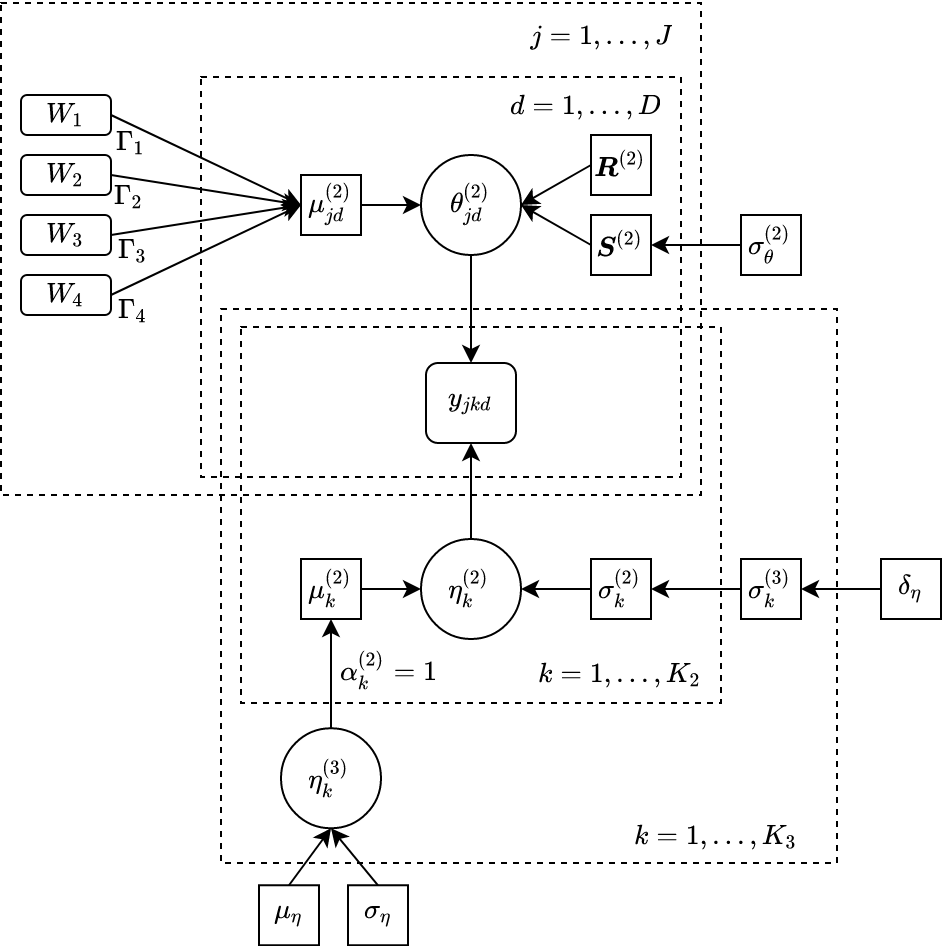
\includegraphics[width=0.7\linewidth]{4_FOLV_dag}
	%
	\caption[Directed Acyclig Graph (DAG). First-order latent variable model (FOLV).]%
	{Directed Acyclig Graph (DAG). First-order latent variable model (FOLV). Circles represent latent variables. Squares represent parameters or parameters for priors. Large squares represent nesting in specific units.}
	\label{fig:FOLV_model}
\end{figure}

Therefore, first, the author selected three different samples sizes to generate the data under analysis: $500$, $250$, and $100$. The literature on IRT models present several implementations with samples sizes above $250$, however, few present samples lower than that. The author decided to use a sample size of a $100$ to fill in this gap. Moreover, the decision was also supported by the notion that the change of the posterior sampling geometries could benefit the performance and recovery capacity of the implementation, under this setting.

Second, as expected, the author used two parametrization of the models: CP and NCP. To the author's knowledge, the IRT literature has not evaluated the change of posterior sampling geometries, as an alternative to improve the performance of the bayesian implementation of said models. The study is set to fill in part of this gap.

Third, the author evaluated the performance, recovery capacity and retrodictive accuracy of a first- and second-order latent variable models; FOLV and SOLV, respectively.

Consequently, ten ($10$) data sets were generated for each study condition, following the algorithm in section \ref{sect:algorithm}. Each data set resembled responses to $25$ binary scored items, conforming to the SOLV model defined in figure \ref{fig:SOLV_model}. The model was motivated by the hypothesized structure of the reading comprehension sub-test, from the Peruvian public teaching career national assessment (see chapter \ref{chap:application}). Finally, the latent structure, regression parameters, and loadings remained unchanged throughout the simulation replicas, to reduce experimental error \cite{Kieftenbeld_et_al_2012}. 
%
\begin{figure}[h]
	\centering
	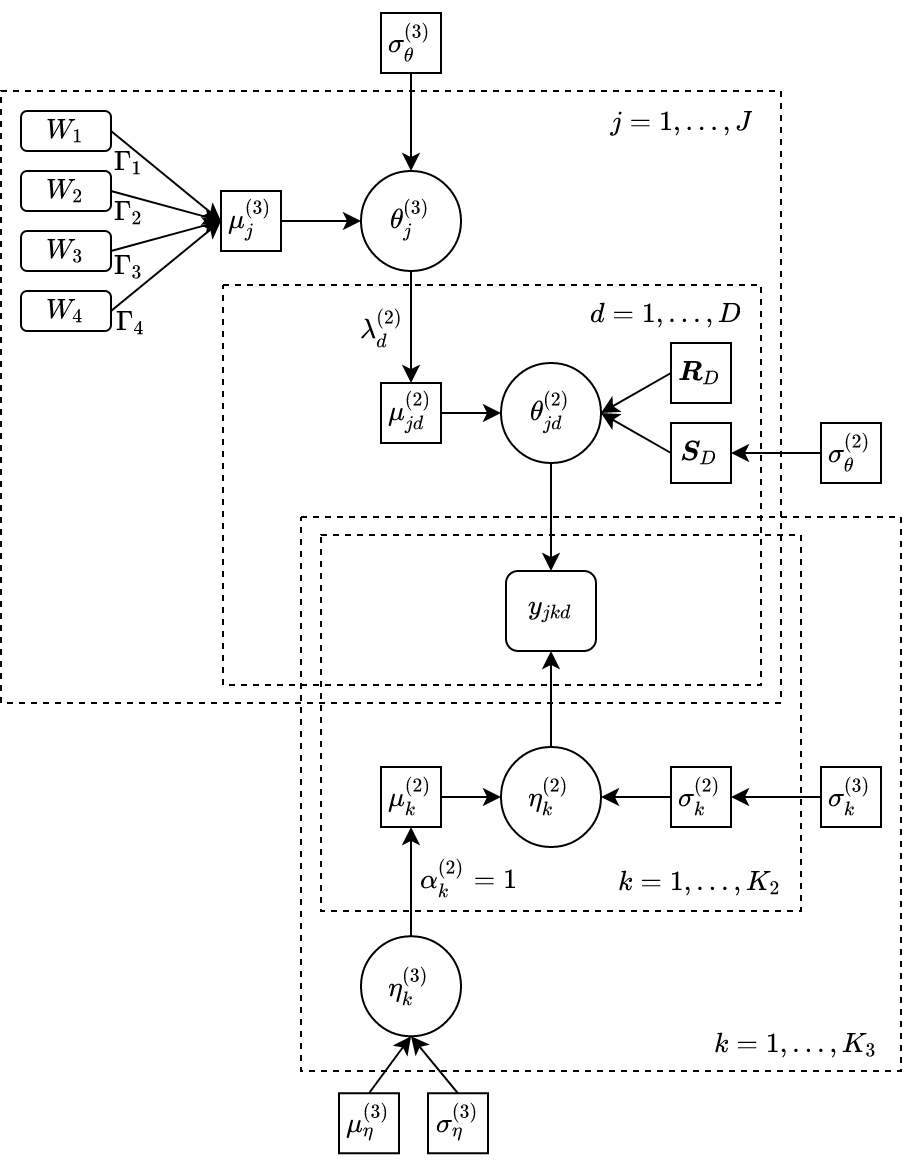
\includegraphics[width=0.8\linewidth]{4_SOLV_dag}
	%
	\caption[Directed Acyclic Graph (DAG). Second-order latent variable model (SOLV).]%
	{Directed Acyclig Graph (DAG). Second-order latent variable model (SOLV). Circles represent latent variables. Squares represent parameters or parameters for priors. Large squares represent nesting in specific units.}
	\label{fig:SOLV_model}
\end{figure}

%%%%%%%%%%%%%%%%%%%%%%%%%%%%%%%%%%%%%%%%%%%%%%%%%%%%%%%%%%%%%%%%%%%%%%%

\section{Algorithm} \label{sect:algorithm}

Each data replication was simulated following a six-step procedure. First, the author randomly simulated a collection of pseudo-covariates $\mathbf{W}_{\theta} = [ W_{1}, W_{2}, W_{3}, W_{4} ]$, motivated by a similar information set present in the reading comprehension sub-test. The generated covariates were: (i) a binary ``gender" variable ($W_{1}$), describing males and females, (ii) an integer ``age" variable ($W_{2}$) with range $[30, 65]$, the latter corresponding to the peruvian age of retirement from the public teacher career, (iii) a three-level categorical ``education" variable ($W_{3}$), indicating the type of education the individual received: institute only, university only, or both; and finally, (iv) a four-level categorical ``experience" variable ($W_{4}$), denoting the individual's years of work experience, where the higher the category, the higher the years of experience. Associated with these, the author defined their regression parameters $\mathbf{\Gamma}_{\theta} = [\Gamma_{0}, \Gamma_{1}, \Gamma_{2}, \Gamma_{3}, \Gamma_{4}]$ where: (i) $\Gamma_{0} = 0$, indicating the absence of an intercept; (ii) $\Gamma_{1} = [\gamma_{m}, \gamma_{f}] = [0, 0.5]$, for males and females, respectively; (iii) $\Gamma_{2} = -0.02$, indicating the individuals loose ability with age, in a linear manner; (iv) $\Gamma_{3} = [\gamma_{io}, \gamma_{uo}, \gamma_{b}] = [-0.5, 0.5, 0]$, assuming individuals with university degree have better ability levels, followed by individuals with both educations, and individuals with institute degrees; and lastly (v) $\Gamma_{4} = [\gamma_{0y}, \gamma_{5y}, \gamma_{10y}, \gamma_{11+y}] = [-0.5, 0, 0.35, 0.5]$, implying experience has decreasing returns on abilities.

Second, the study simulated the second- and first-order latent variables, corresponding to the reading comprehension ability and its three sub-dimensions: literal, inferential and reflective. Reading comprehension ($\theta^{(3)}_{j}$) was generated from a normal distribution $N( \mu^{(3)}_{j}, \sigma^{(3)}_{\theta} )$, with $\mu^{(3)}_{j} = \pmb{\Gamma}_{\theta} \; \mathbf{W}_{\theta}$, that is, the linear combination of the simulated covariates and its corresponding regression parameters, and $\sigma^{(3)}_{\theta}=0.5$. On the other hand, the three sub-dimensions were generated from a multivariate normal distribution $MVN( \pmb{\mu}^{(2)}_{j} , \pmb{\Sigma}^{(2)})$, with a mean vector $\pmb{\mu}^{(2)}_{j} = [\mu^{(2)}_{j1}, \mu^{(2)}_{j2}, \mu^{(2)}_{j3}] = [\lambda^{(2)}_{1} \theta^{(3)}_{j}, \; \lambda^{(2)}_{2} \theta^{(3)}_{j}, \; \lambda^{(2)}_{3} \theta^{(3)}_{j} ]$, loadings $\pmb{\lambda}^{(2)} = [\lambda^{(2)}_{1}, \lambda^{(2)}_{2}, \lambda^{(2)}_{3}] = [0.95, 0.95, 0.95]$, and a factored covariance matrix $\pmb{\Sigma}^{(2)} = \mathbf{S}^{(2)} \cdot \mathbf{R}^{(2)} \cdot \mathbf{S}^{(2)}$; where $\mathbf{S}^{(2)} = \pmb{\sigma}^{(2)}_{\theta} \mathbf{I}$ is a diagonal standard deviation matrix with $\pmb{\sigma}^{(2)}_{\theta} = [0.5, 0.5, 0.5]$, whereas $\mathbf{R}^{(2)} = \mathbf{I}$ is an identity correlation matrix, implying the simulated sub-dimensions are independent, after accounting for the reading comprehension.

Third, the author defined five ($5$) common stimulus or texts for the items, where the mean difficulty for the texts $\pmb{\eta}^{(3)} = [\eta^{(3)}_{1}, \eta^{(3)}_{2}, \eta^{(3)}_{3}, \eta^{(3)}_{4}, \eta^{(3)}_{5}] = [-1.50, -0.75, 0, 0.75, 1.50]$; whereas the deviation from said mean difficulties were $\sigma^{(3)}_{k} = 0.5$ for all texts. 

Fourth, $25$ items were randomly generated from independent normal distributions $N( \mu^{(2)}_{k}, \sigma^{(2)}_{k} ) $, with $\mu^{(2)}_{k} = \pmb{\eta}^{(3)} \pmb{\alpha}^{(2)} \mathbf{A}$ and $\sigma^{(2)}_{k} = \sigma^{(3)}_{k}$; where $\pmb{\alpha}^{(2)} = \mathbf{1}$, indicating the difficulty of the common stimulus directly explained the difficulty of the items, and $\mathbf{A}$ was a block design matrix that maps the items to its corresponding passage. Lastly, the items' measured dimensions were also generated at random, for each replica.

Fifth, the author calculated the linear predictor $v_{jkd}$ and probability of endorsing an item $\pi_{jkd}$ according to equations (\ref{eq:systematic}), (\ref{eq:response_dich1}), and (\ref{eq:linear_predictor2}), respectively. The probabilities were calculated using the logistic inverse-link function.
	
Sixth and last, the outcome $y_{jkd}$ was simulated from a Bernoulli distribution as in equation (\ref{eq:distributional}), with a probability of success calculated as in the previous step. 

The code associated with the full simulation process can be found in Appendix \ref{appC2_1:sim}.

%%%%%%%%%%%%%%%%%%%%%%%%%%%%%%%%%%%%%%%%%%%%%%%%%%%%%%%%%%%%%%%%%%%%%%%
%%%%%%%%%%%%%%%%%%%%%%%%%%%%%%%%%%%%%%%%%%%%%%%%%%%%%%%%%%%%%%%%%%%%%%%

\section{Evaluation criteria}

As stated in the objectives, the study was set to evaluate the performance, recovery capacity, and retrodictive accuracy of the bayesian implementation.

First, to assess the performance of the MCMC chains, in terms of achieving stationarity, convergence and good mixing, the author followed the usual bayesian approach. The approach involved the visual evaluation of trace plots, for stationarity and convergence (more useful to establish lack of thereof); and trank and autocorrelation plots (ACF), for good mixing. Moreover, the assessment of convergence and mixing were supported by the \textit{potential scale reduction factor} (\texttt{Rhat}) and \textit{effective sample size} (\texttt{n\_eff}) statistics developed by \citet{Gelman_et_al_2014} (pp. $284-287$).

Second, to evaluate the recovery capacity for all the parameters $\pmb{\Omega} = \{ \pmb{\beta}, \pmb{\Lambda}, \pmb{\Theta}, \pmb{\Psi}, \pmb{\Gamma} \}$, we used the between replica root mean squared error ($\text{RMSE}_{B}$), i.e. the extent of the deviation the posterior means exhibited from the true generating values, in all replicate simulations. The $\text{RMSE}_{B}$ for each parameter of interest was defined as follows:
%
\begin{align}
	%
	\text{RMSE}_{B} \left( \eta^{(m)}_{k} \right) &=\sqrt{\frac{1}{R} \sum_{r=1}^{R} \left( \frac{1}{S} \sum_{s=1}^{S} \hat{\eta}^{(m)}_{krs} - \eta^{(m)}_{k} \right)^2}
	%
\end{align}
%
\begin{align}
	%
	\text{RMSE}_{B} \left( \theta^{(l)}_{jd} \right) &=\sqrt{\frac{1}{R} \sum_{r=1}^{R} \left( \frac{1}{S} \sum_{s=1}^{S} \hat{\theta}^{(l)}_{jdrs} - \theta^{(l)}_{jd} \right)^2} 
	%
\end{align}
%
\begin{align}
	%
	\text{RMSE}_{B} \left( \Gamma_{w} \right) &=\sqrt{\frac{1}{R} \sum_{r=1}^{R} \left( \frac{1}{S} \sum_{s=1}^{S} \hat{\Gamma}_{wrs} - \Gamma_{w} \right)^2}
	%
\end{align}
%
\begin{align}
	%
	\text{RMSE}_{B} \left( \lambda^{(l)}_{d} \right) &=\sqrt{\frac{1}{R} \sum_{r=1}^{R} \left( \frac{1}{S} \sum_{s=1}^{S} \hat{\lambda}^{(l)}_{drs} - \lambda^{(l)}_{d} \right)^2}
	%
\end{align}

%
\begin{align}
	%
	\text{RMSE}_{B} \left( \rho^{(2)}_{dq} \right) &=\sqrt{\frac{1}{R} \sum_{r=1}^{R} \left( \frac{1}{S} \sum_{s=1}^{S} \hat{\rho}^{(2)}_{dqrs} - \rho^{(2)}_{dq} \right)^2}
	%
\end{align}

\noindent where the ``hat" parameters with index $rs$ described the parameter's posterior sample $s=1, \dots, S$, with $S=3,000$; and replica $r=1, \dots, R$, with $R=10$. Additionally, $\rho^{(2)}_{dq}$ denoted the dimensions' correlation parameters in matrix $\boldsymbol{R}^{(2)}$, with $q>d$, where $d=1,\dots,3$ and $q=1,\dots,3$. Notice in the case of the FOLV model, in order to asses the recovery capacity of the correlations, we were forced to calculate an approximate implied correlation structure between sub-dimensions, resulting from having a miss-specified model. The calculation was perform through the use of Wright's tracing rules \cite{Beaujean_2014}.

Finally, since IRT models are known to be invariant to the shift of the linear predictor \cite{Baker_et_al_1992, Bock_1972}, i.e. the addition/subtraction of a constant to the abilities/difficulties results in the same probability value, it could happen that we observe substantial differences in the recovery of the parameters, that not necessarily implies a classification error  \cite{Wollack_2002}. Therefore, to avoid a mistake in the model's assessment of fit, the current research will use posterior predictive checks, i.e. we use the parameters' posterior distribution to asses how good is the retrodictive accuracy of the implementation.

The retrodictive accuracy was measured by the root mean squared error of the responses' predictive proportion $\hat{p}$, versus the observed proportion $p$, according to a set of aggregating dimensions. However, since there is prediction uncertainty within and between replicas, we defined two measures:
%
\begin{align}
	%
	\overline{\text{RMSE}}_{W} \left( p_{j} \right) &= \frac{1}{R} \sum_{r=1}^{R} \sqrt{ \frac{1}{S} \sum_{s=1}^{S} \left( \hat{p}_{jrs} - p_{j} \right)^2} \\
	%
	\text{RMSE}_{B} \left( p_{j} \right) &= \sqrt{ \frac{1}{R} \sum_{r=1}^{R}  \left( \frac{1}{S} \sum_{s=1}^{S} \hat{p}_{jrs} - p_{j} \right)^2} 
	%
\end{align}

\noindent where $\overline{\text{RMSE}}_{W}$ and $\text{RMSE}_{B}$ denotes the average within and between prediction root mean squared error, respectively; while $j=1,\dots,J$ defined the individual's index, $S=3,000$ and $R=10$. Notice from the previous equations that we obtain two measures of deviations from the true proportion, per individual.

In a similar manner, we calculated the statistics for each item, text, dimension, and even per each individual and simulated covariate combination. Such statistics were defined as follows:
%
\begin{align}
	%
	\overline{\text{RMSE}}_{W} \left( p_{k} \right) &= \frac{1}{R} \sum_{r=1}^{R} \sqrt{ \frac{1}{S} \sum_{s=1}^{S} \left( \hat{p}_{krs} - p_{k} \right)^2} \\
	%
	\text{RMSE}_{B} \left( p_{k} \right) &= \sqrt{ \frac{1}{R} \sum_{r=1}^{R}  \left( \frac{1}{S} \sum_{s=1}^{S} \hat{p}_{krs} - p_{k} \right)^2} 
	%
\end{align}
%
\begin{align}
	%
	\overline{\text{RMSE}}_{W} \left( p_{l} \right) &= \frac{1}{R} \sum_{r=1}^{R} \sqrt{ \frac{1}{S} \sum_{s=1}^{S} \left( \hat{p}_{lrs} - p_{l} \right)^2} \\
	%
	\text{RMSE}_{B} \left( p_{l} \right) &= \sqrt{ \frac{1}{R} \sum_{r=1}^{R}  \left( \frac{1}{S} \sum_{s=1}^{S} \hat{p}_{lrs} - p_{l} \right)^2} 
	%
\end{align}
%
\begin{align}
	%
	\overline{\text{RMSE}}_{W} \left( p_{d} \right) &= \frac{1}{R} \sum_{r=1}^{R} \sqrt{ \frac{1}{S} \sum_{s=1}^{S} \left( \hat{p}_{drs} - p_{d} \right)^2} \\
	%
	\text{RMSE}_{B} \left( p_{d} \right) &= \sqrt{ \frac{1}{R} \sum_{r=1}^{R}  \left( \frac{1}{S} \sum_{s=1}^{S} \hat{p}_{drs} - p_{d} \right)^2} 
	%
\end{align}
%
\begin{align}
	%
	\overline{\text{RMSE}}_{W} \left( p_{jw} \right) &= \frac{1}{R} \sum_{r=1}^{R} \sqrt{ \frac{1}{S} \sum_{s=1}^{S} \left( \hat{p}_{jwrs} - p_{jw} \right)^2} \\
	%
	\text{RMSE}_{B} \left( p_{jw} \right) &= \sqrt{ \frac{1}{R} \sum_{r=1}^{R}  \left( \frac{1}{S} \sum_{s=1}^{S} \hat{p}_{jwrs} - p_{jw} \right)^2} 
	%
\end{align}

\noindent where $k= 1, \dots, 25$ items; $l=1, \dots, 5$ texts; $d=1, \dots ,3$ dimensions; and $w=1, \dots, 4$ simulated covariates.

%%%%%%%%%%%%%%%%%%%%%%%%%%%%%%%%%%%%%%%%%%%%%%%%%%%%%%%%%%%%%%%%%%%%%%%
%%%%%%%%%%%%%%%%%%%%%%%%%%%%%%%%%%%%%%%%%%%%%%%%%%%%%%%%%%%%%%%%%%%%%%%

\section{Parameter estimation}

\subsection{Likelihood, priors and hyper-priors}

As stated in previous sections, we analyzed two models, that is, the FOLV model depicted in figure \ref{fig:FOLV_model}, and the SOLV model depicted in figure \ref{fig:SOLV_model}. In this section, we proceed to enumerate the likelihood functions, and the full set of priors and \textit{hyper-priors} used, for the centered and non-centered parametrizations, respectively.

First, for the centered parametrization (CP), as stated in equations (\ref{eq:lin_pred}), (\ref{eq:prob}), and (\ref{eq:dist}), the distributional and systematic part of both models was defined as follows:
%
\begin{align}
	%
	y_{jkd} &\sim \text{Bernoulli}( \pi_{jkd} ) \\
	%
%\end{align}
%
%\begin{align}
	%
	\text{logit}( \pi_{jkd} ) &= v_{jkd} \\
	%
	v_{jkd} &= \theta^{(2)}_{jd} - \eta^{(2)}_{k}
	%
\end{align}

Notice the linear predictor can be considered a multilevel-multidimensional extension of the well known Rasch IRT model \cite{Rasch_1980}. The first-order latent variables were defined as follows:
%
\begin{align}
	%
	\boldsymbol{\theta}^{(2)}_{j} &= \left[ \theta_{j1}^{(2)}, \theta_{j2}^{(2)}, \theta_{j3}^{(2)} \right] \\
	%
	\boldsymbol{\theta}^{(2)}_{j} &\sim \text{MVNormal} \left( \boldsymbol{\mu}^{(2)}_{j}, \boldsymbol{\Sigma}^{(2)} \right) \label{eq:theta_sub}
	%
\end{align}

\noindent where $\boldsymbol{\Sigma}^{(2)}$ was defined by a factorization of the variances and correlations structures, in the following form:
%
\begin{align} \label{eq:sigma_factoring}
	%
	\boldsymbol{\Sigma}^{(2)} &= \boldsymbol{S}^{(2)} \cdot \boldsymbol{R}^{(2)} \cdot \boldsymbol{S}^{(2)} \\
	%
	\boldsymbol{S}^{(2)} = \pmb{\sigma}^{(2)}_{\theta} \mathbf{I} &= 
	\begin{pmatrix}
		\sigma^{2}_{1}	& 0 			 	& 0 				\\
		0 				& \sigma^{2}_{2} 	& 0 				\\
		0 				& 0					& \sigma^{2}_{3} 
	\end{pmatrix} \label{eq:sigmas}\\
	%
	\boldsymbol{R}^{(2)} &= 
	\begin{pmatrix}
		1			& \rho_{12} & \rho_{13} 	\\
		\rho_{21} 	& 1 		& \rho_{23} 	\\
		\rho_{31} 	& \rho_{32}	& 1	
	\end{pmatrix} 
	%
\end{align}

\noindent while $\boldsymbol{\mu}^{(2)}_{j}$ was defined in two ways, depending on the model we were fitting. For the FOLV model, the mean vector was defined as follows:
%
\begin{align}
	%
	\boldsymbol{\mu}^{(2)}_{j} &= \left[ \mu^{(2)}_{j1}, \; \mu^{(2)}_{j2}, \mu^{(2)}_{j3} \right] \label{eq:mu_FOLV} \\
	%
	\mu^{(2)}_{jd} &= \Gamma_{0} + \Gamma_{1} W_{1j} + \Gamma_{2} (W_{2j} - W_{2\text{min}}) + \Gamma_{3} W_{3j} + \Gamma_{4} W_{4j}
	%
\end{align}

\noindent where $\Gamma_{p}$ and $W_{jp}$ are defined as in section \ref{sect:algorithm}. Notice the regression parameters were not dimension specific. On the other hand, for the SOLV model, $\boldsymbol{\mu}^{(2)}_{j}$ was defined by:
%
\begin{align}
	%
	\boldsymbol{\mu}^{(2)}_{j} &= \left[ \mu^{(2)}_{j1}, \; \mu^{(2)}_{j2}, \mu^{(2)}_{j3} \right] \\
	%
	\pmb{\lambda}^{(2)} &= \left[ \lambda^{(2)}_{1}, \; \lambda^{(2)}_{2}, \lambda^{(2)}_{3} \right] \\
	%
	\mu^{(2)}_{jd} &= \lambda^{(2)}_{d} \; \theta^{(3)}_{j} 
	%
\end{align}

\noindent where $d$ denoted the index of the individual's dimension. Lastly, because the SOLV contemplates an additional level, corresponding to the reading comprehension ability, an additional set of parameters was defined as follows:
%
\begin{align}
	%
	\theta^{(3)}_{j} &\sim \text{Normal} \left( \mu^{(3)}_{j}, \sigma^{(3)}_{\theta} \right) \label{eq:theta} \\
	%
	\mu^{(3)}_{j} &=  \Gamma_{0} + \Gamma_{1} W_{1j} + \Gamma_{2} (W_{2j} - W_{2\text{min}}) + \Gamma_{3} W_{3j} + \Gamma_{4} W_{4j} \label{eq:mu_SOLV}
\end{align}

Turning now our attention to the items' parameters $\eta^{(2)}_{k}$, both models had:
%
\begin{align}
	%
	\eta^{(2)}_{k} &\sim \text{Normal} \left( \mu^{(2)}_{k}, \sigma^{(2)}_{k} \right) \label{eq:items} \\
	%
	\mu^{(2)}_{k} &= \pmb{\eta}^{(3)} \mathbf{A} \label{eq:mu_items} \\
	%
	\sigma^{(2)}_{k} &= \pmb{\sigma}^{(3)} \mathbf{A} \label{eq:sigma_items}
	%
\end{align}

\noindent where $k=1, \dots, 25$ items, $\pmb{\eta}^{(3)} = [ \eta^{(3)}_{1}, \eta^{(3)}_{2}, \eta^{(3)}_{3}, \eta^{(3)}_{4}, \eta^{(3)}_{5} ]$ represented the texts difficulties, $\pmb{\sigma}^{(3)} = [ \sigma^{(3)}_{1}, \sigma^{(3)}_{2}, \sigma^{(3)}_{3}, \sigma^{(3)}_{4}, \sigma^{(3)}_{5} ]$ the text deviations from such difficulties; and $\mathbf{A}$ was a block design matrix that mapped the items to its corresponding passage. In addition, $\eta^{(3)}_{k}$ and $\sigma^{(3)}_{k}$ were distributed as follows:
%
\begin{align}
	%
	\eta^{(3)}_{k} &\sim \text{Normal} \left( \mu_{\eta}, \sigma_{\eta} \right) \\
	%
	\sigma^{(3)}_{k} &\sim \text{Exponential} \left( \delta_{\eta} \right)
	%
\end{align}

Lastly, we declare the remaining prior and \textit{hyper-priors} in the following form::
%
\begin{align}
	\boldsymbol{R}^{(2)} &\sim \text{LkjCorrelation}( 2 ) \\
	\beta_{G} &\sim \text{Normal}( 0, 0.5 ) \\
	\beta_{A} &\sim \text{Normal}( 0, 0.5 ) \\
	\beta_{E} &\sim \text{Normal}( 0, 1 ) \\
	\beta_{X} &\sim \text{Normal}( 0, 0.5 ) 
	%
\end{align}

\noindent where $\text{LKJCorrelation}(\cdot)$ denotes the Lewandowski, Kurowicka, and Joe prior correlation distribution \cite{Lewandowski_et_al_2009}. Notice from equation (\ref{eq:sigma_factoring}), and the aforementioned prior, that the current research departs from the usual setting of prior distributions for covariances matrices. As it is point out by \citet{Depaoli_2021}, the literature on bayesian MSEM/CFA/IRT have favored the use of the Inverse-Wishart distribution, as a prior for covariances matrices, based on its conjugancy properties. However, the assumptions derived from its use, that is, the priors are equally informative for variances and covariances, is sometimes restrictive. Therefore, following \citet{McElreath_2020}, we believe that by factoring the covariance matrix into variances and correlations, allow us gain control on the preliminary assumptions set to those parameters. Moreover, it makes easier to identify when the researcher is using the unit variance identification scheme (UVI, see next section); and allow us to transition easily to the non-centered parametrization (NCP).

Second, as it was outlined in section \ref{subsub_sec:NCP}, to identify parameters that can be transformed into the NCP, we needed to recognize equations where the parameters' sampling procedure is dependent on other sampled parameters. A careful inspection of the preceding parametrization revealed that equations (\ref{eq:theta_sub}), (\ref{eq:theta}), and (\ref{eq:items}) fulfilled this characteristic. Therefore, under the NCP, equation (\ref{eq:items}) was re-defined as follows:
%
\begin{align}
	%
	\eta^{(2)}_{k} &= \mu^{(2)}_{k} + \sigma^{(2)}_{k} z^{(2)}_{k} \\
	%
	z^{(2)}_{k} &\sim \text{Normal}(0,1)
	%
\end{align}

\noindent where $\mu^{(2)}_{k}$ and $\sigma^{(2)}_{k}$ are defined as in equations (\ref{eq:mu_items}) and (\ref{eq:sigma_items}), respectively; while $z^{(2)}_{k}$ was sampled from independent standard normal distributions, one for each item corresponding to a text passage.

Moreover, equation (\ref{eq:theta_sub}) was re-defined as follows:
%
\begin{align}
	%
	\boldsymbol{\theta}^{(2)}_{j} &= \boldsymbol{\mu}^{(2)}_{j} + \boldsymbol{S}^{(2)} \cdot \boldsymbol{L}^{(2)}_{\Sigma} \cdot  (\mathbf{z}_{j} \mathbf{I}) \\
	%
	\mathbf{z}_{j} &= [ z_{j1}, \dots, z_{jd}]^{T}
	%
\end{align}

\noindent where $\boldsymbol{\mu}^{(2)}_{j}$ is defined as in equation (\ref{eq:mu_FOLV}), $\boldsymbol{S}^{(2)}$ is defined as in equation (\ref{eq:sigmas}), and $\mathbf{I}$ is an identity matrix. Additionally, we had:
%
\begin{align}
	%
	z_{jd} &\sim \text{Normal}(0,1) \\
	%
	\boldsymbol{L}^{(2)}_{\Sigma} &\sim \text{LKJCorrelationCholesky}(2)
	%
\end{align}

\noindent where $z_{jd}$ was sampled from independent standard normal distributions (one for each dimension and individual); while $\boldsymbol{L}^{(2)}_{\Sigma}$ denoted the Cholesky factorization of the correlation matrix $\boldsymbol{R}^{(2)}$. A Cholesky factorization is a decomposition of any positive-definite matrix $\mathbf{A}$, into the product of a lower triangular matrix and its conjugate transpose, i.e. $\mathbf{A} = \boldsymbol{L} \cdot \boldsymbol{L}^{T}$. Notice the prior distribution of the decomposition $\text{LKJCorrelationCholesky}(\cdot)$, implied the same assumption as before, that is, $\boldsymbol{R}^{(2)} = \boldsymbol{L}^{(2)}_{\Sigma} \cdot \boldsymbol{L}^{(2)T}_{\Sigma} \sim  \text{LKJCorrelation}(2)$\footnote{See \citet{Stan2020} for a detailed explanation on the implementation.}.

Furthermore, as in the previous cases, equation (\ref{eq:theta}) also shows sampling dependence. Therefore, the equation was re-defined as follows:
%
\begin{align}
	%
	\theta^{(3)}_{j} &= \mu^{(3)}_{j} + \sigma^{(3)}_{\theta} z_{j} \\
	%
	z_{j} &\sim \text{Normal}(0,1)
	%
\end{align}

\noindent where $\mu^{(3)}_{j}$ is defined as in equation (\ref{eq:mu_SOLV}), and $z_{j}$ was sampled from independent standard normal distributions, one for each individual. Finally, the remaining equations defined under the CP maintain their description under the NCP.

%%%%%%%%%%%%%%%%%%%%%%%%%%%%%%%%%%%%%%%%%%%%%%%%%%%%%%%%%%%%%%%%%%%%%%%

\subsection{Identification}

In order to fully specify the model and provide a scale for the latent variables, we decided to use the UVI scheme, that is, to set the scale of the higher-order dimension and sub-dimensions to one,  $\sigma^{(3)}_{\theta} = 1$ and $\mathbf{S}^{(2)} = \pmb{\sigma}^{(2)}_{\theta} \mathbf{I}$ with $\pmb{\sigma}^{(2)}_{\theta} = [1, 1, 1]^{T}$. The previous effectively turned the covariance matrix $\boldsymbol{\Sigma}^{(2)}$ into a correlation, i.e. $\boldsymbol{\Sigma}^{(2)} = \boldsymbol{R}^{(2)}$ (see equation \ref{eq:sigma_factoring}). Moreover, we identified the texts' and items' by setting $\mu_{\eta} = 0$, $\sigma_{\eta}=1$, $\delta_{\eta}=2$.

Notice we needed to set the scales for all the individuals' dimensions equal to one, because otherwise the latent structure would be under-identified. In either model, at the level of the first-order latent variables (level-2), we would have $(3 \times 4)/2 = 6$ pieces of information available, corresponding to the variances and covariances of the latent variables. Then, the information would need to estimate $10$ parameters, i.e. $3$ loadings, $3$ variances corresponding to the first--order latent variable, $1$ variance for the second-order latent variable (if present), and $3$ correlations among sub-dimensions, making that portion of the model under-identified. Therefore, by restricting the variances to one, we have enough information to estimate other parameters of interest (correlations and loading, if present). Additionally, this is further justified by the fact that latent variables have no inherent unit in which they are measured, consequently, setting their scale is an arbitrary  decision \cite{Beaujean_2014}.


\begin{comment}
On the other hand, from the texts and items perspective, at the level of the items (level-2) we would have $(25 \times 26)/2 = 325$ pieces of information available, corresponding to the variances and covariances of the items dimensions. With that information we would need to estimate $30$ parameters, corresponding to $25$ items' dimension variances, and $5$ texts' dimension variances. notice in this case, we do not need to estimate $25$ loadings, as they are assumed to be $1$.
\end{comment}

%%%%%%%%%%%%%%%%%%%%%%%%%%%%%%%%%%%%%%%%%%%%%%%%%%%%%%%%%%%%%%%%%%%%%%%

\subsection{Prior predictive investigation} \label{sub_sect:prior_pred_inv}

As it was outlined in section \ref{sub_sect:prior_pred}, we will use prior predictive investigation to assess and visualize the consequences of our prior assumptions. The implications will be assessed from two perspectives: the IRT and the outcome space perspective. For the former, we will investigate what the set of priors imply for the item characteristic curves (ICC), and item information function (IIF). For the latter, we will examine how the prior assumption translate onto the outcome space.

First, it will useful to define the ICC and IIF functions. \citet{Hambleton_et_al_1991b} defined the ICC as the mathematical function that relates the probability of success on an item, to the ability measured by that same item. In our current implementation, such function would correspond to the systematic part of the GLLAMM, as defined in equations (\ref{eq:systematic}) and (\ref{eq:response_dich1}):
%
\begin{equation} \label{eq:ICC}
	\begin{split}
		\text{ICC} &= \pi_{jkd} = \frac{ \text{exp}(v_{jkd}) }{ 1 + \text{exp}(v_{jkd}) }
	\end{split}	
\end{equation}

\noindent where the linear predictor $v_{jkd}$ contains the items' difficulties $\eta^{(2)}_{k}$ and the individuals' sub-dimensions/abilities $\theta^{(2)}_{jd}$, as defined in equation (\ref{eq:linear_predictor1}). As previously mentioned, the ICC of our current implementation can be considered as the multilevel-multidimensional extension to the Rasch's ICC.

On the other hand, the same authors defined the IIF as a function that measured the amount of information provided by an item. In this setting, ``information" is understood as the reduction of uncertainty, resulting from using an item to measure the ability of an individual. Given the above, the IIF for the GLLAMM was defined in a similar manner as the Rasch counterpart, in the following form:
%
\begin{equation} \label{eq:IIF}
	\begin{split}
		\text{IIF} &= \pi_{jkd} \; (1 - \pi_{jkd})
	\end{split}	
\end{equation}
%
\begin{figure}[H]
	\centering
	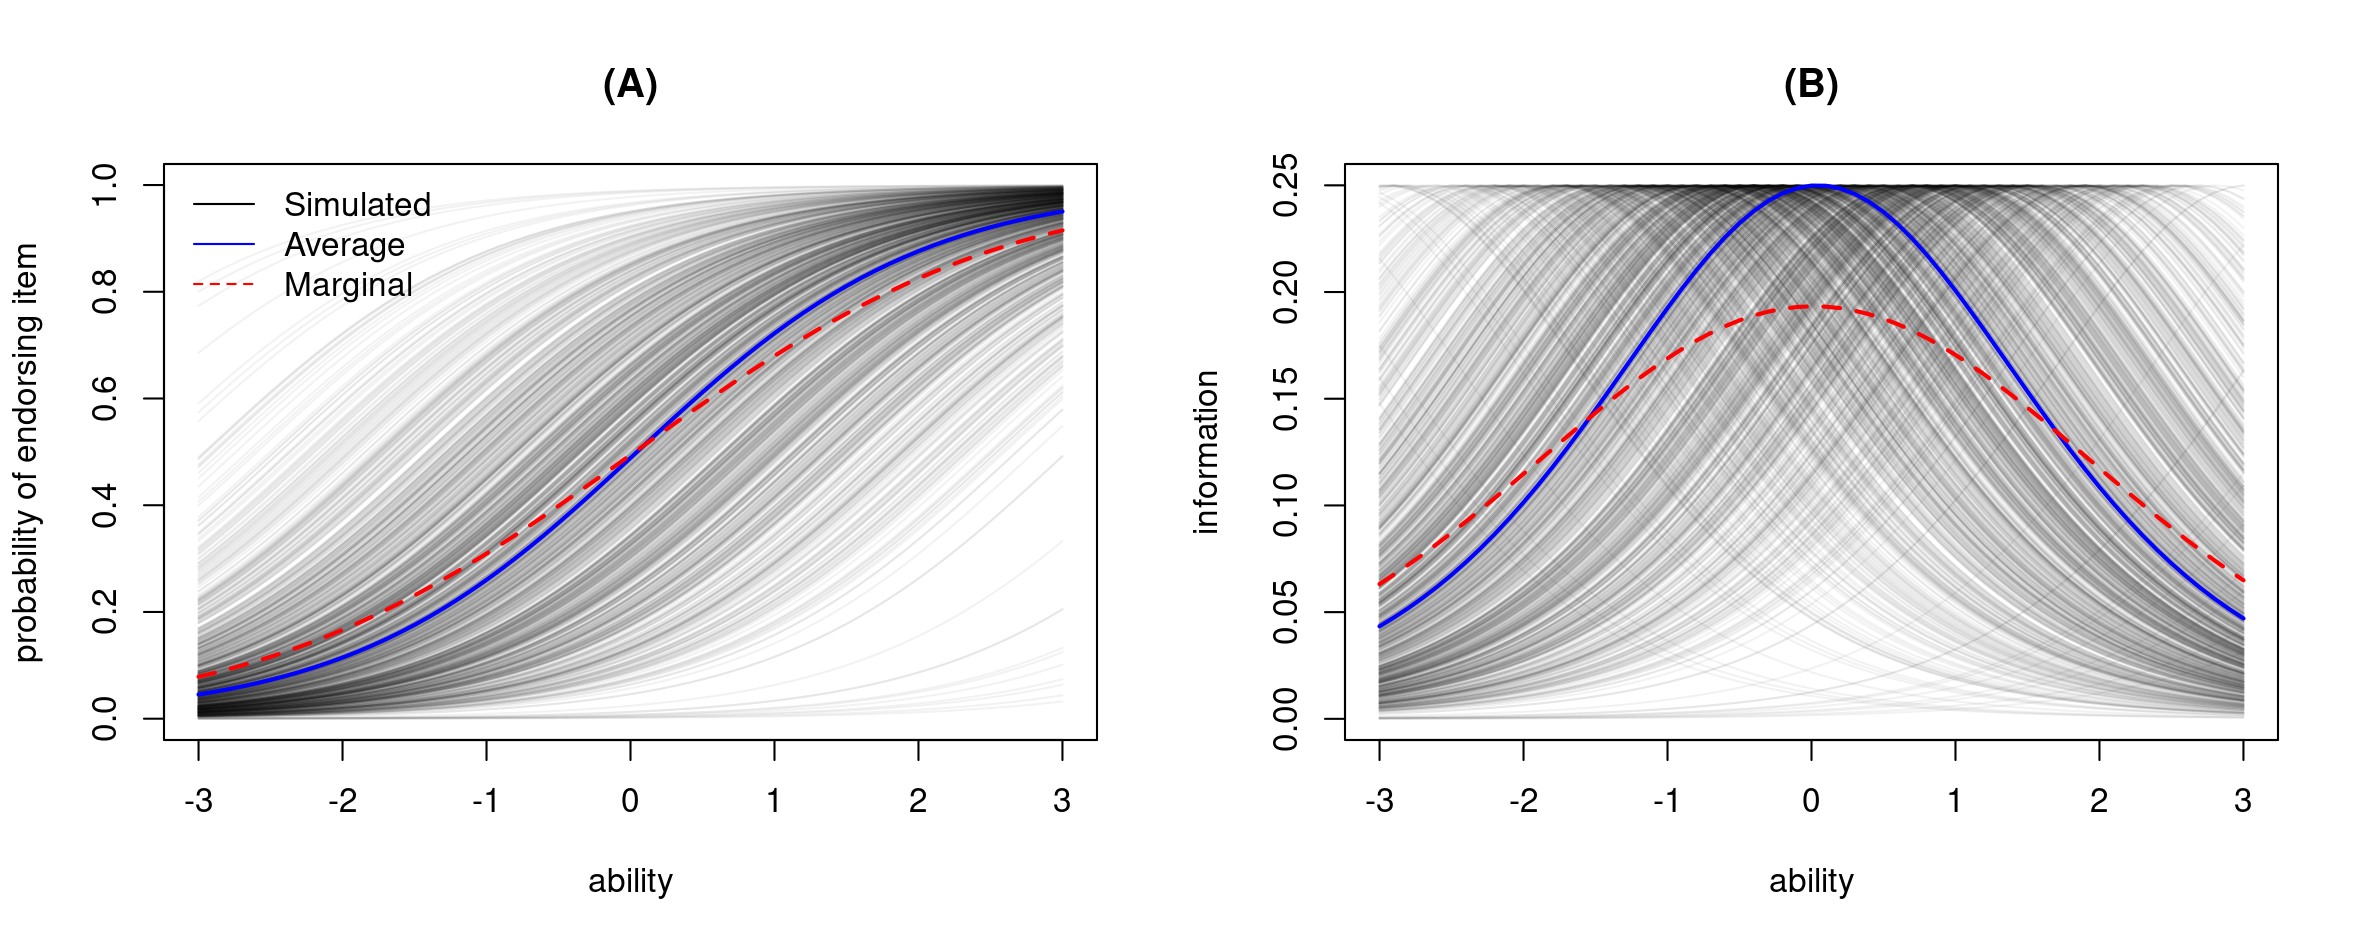
\includegraphics[width=1\linewidth]{FOLV_ICC_prior}
	%
	\caption[First-order latent variable model (FOLV). Item Characteristic Curve (ICC) and Item Information Function (IIF).]%
	{First-order latent variable model (FOLV). (A) Item Characteristics Curve, ICC. (B) Item Information Function, IIF.}
	\label{fig:FOLV_ICC_prior}
\end{figure} 
%
\begin{figure}[H]
	\centering
	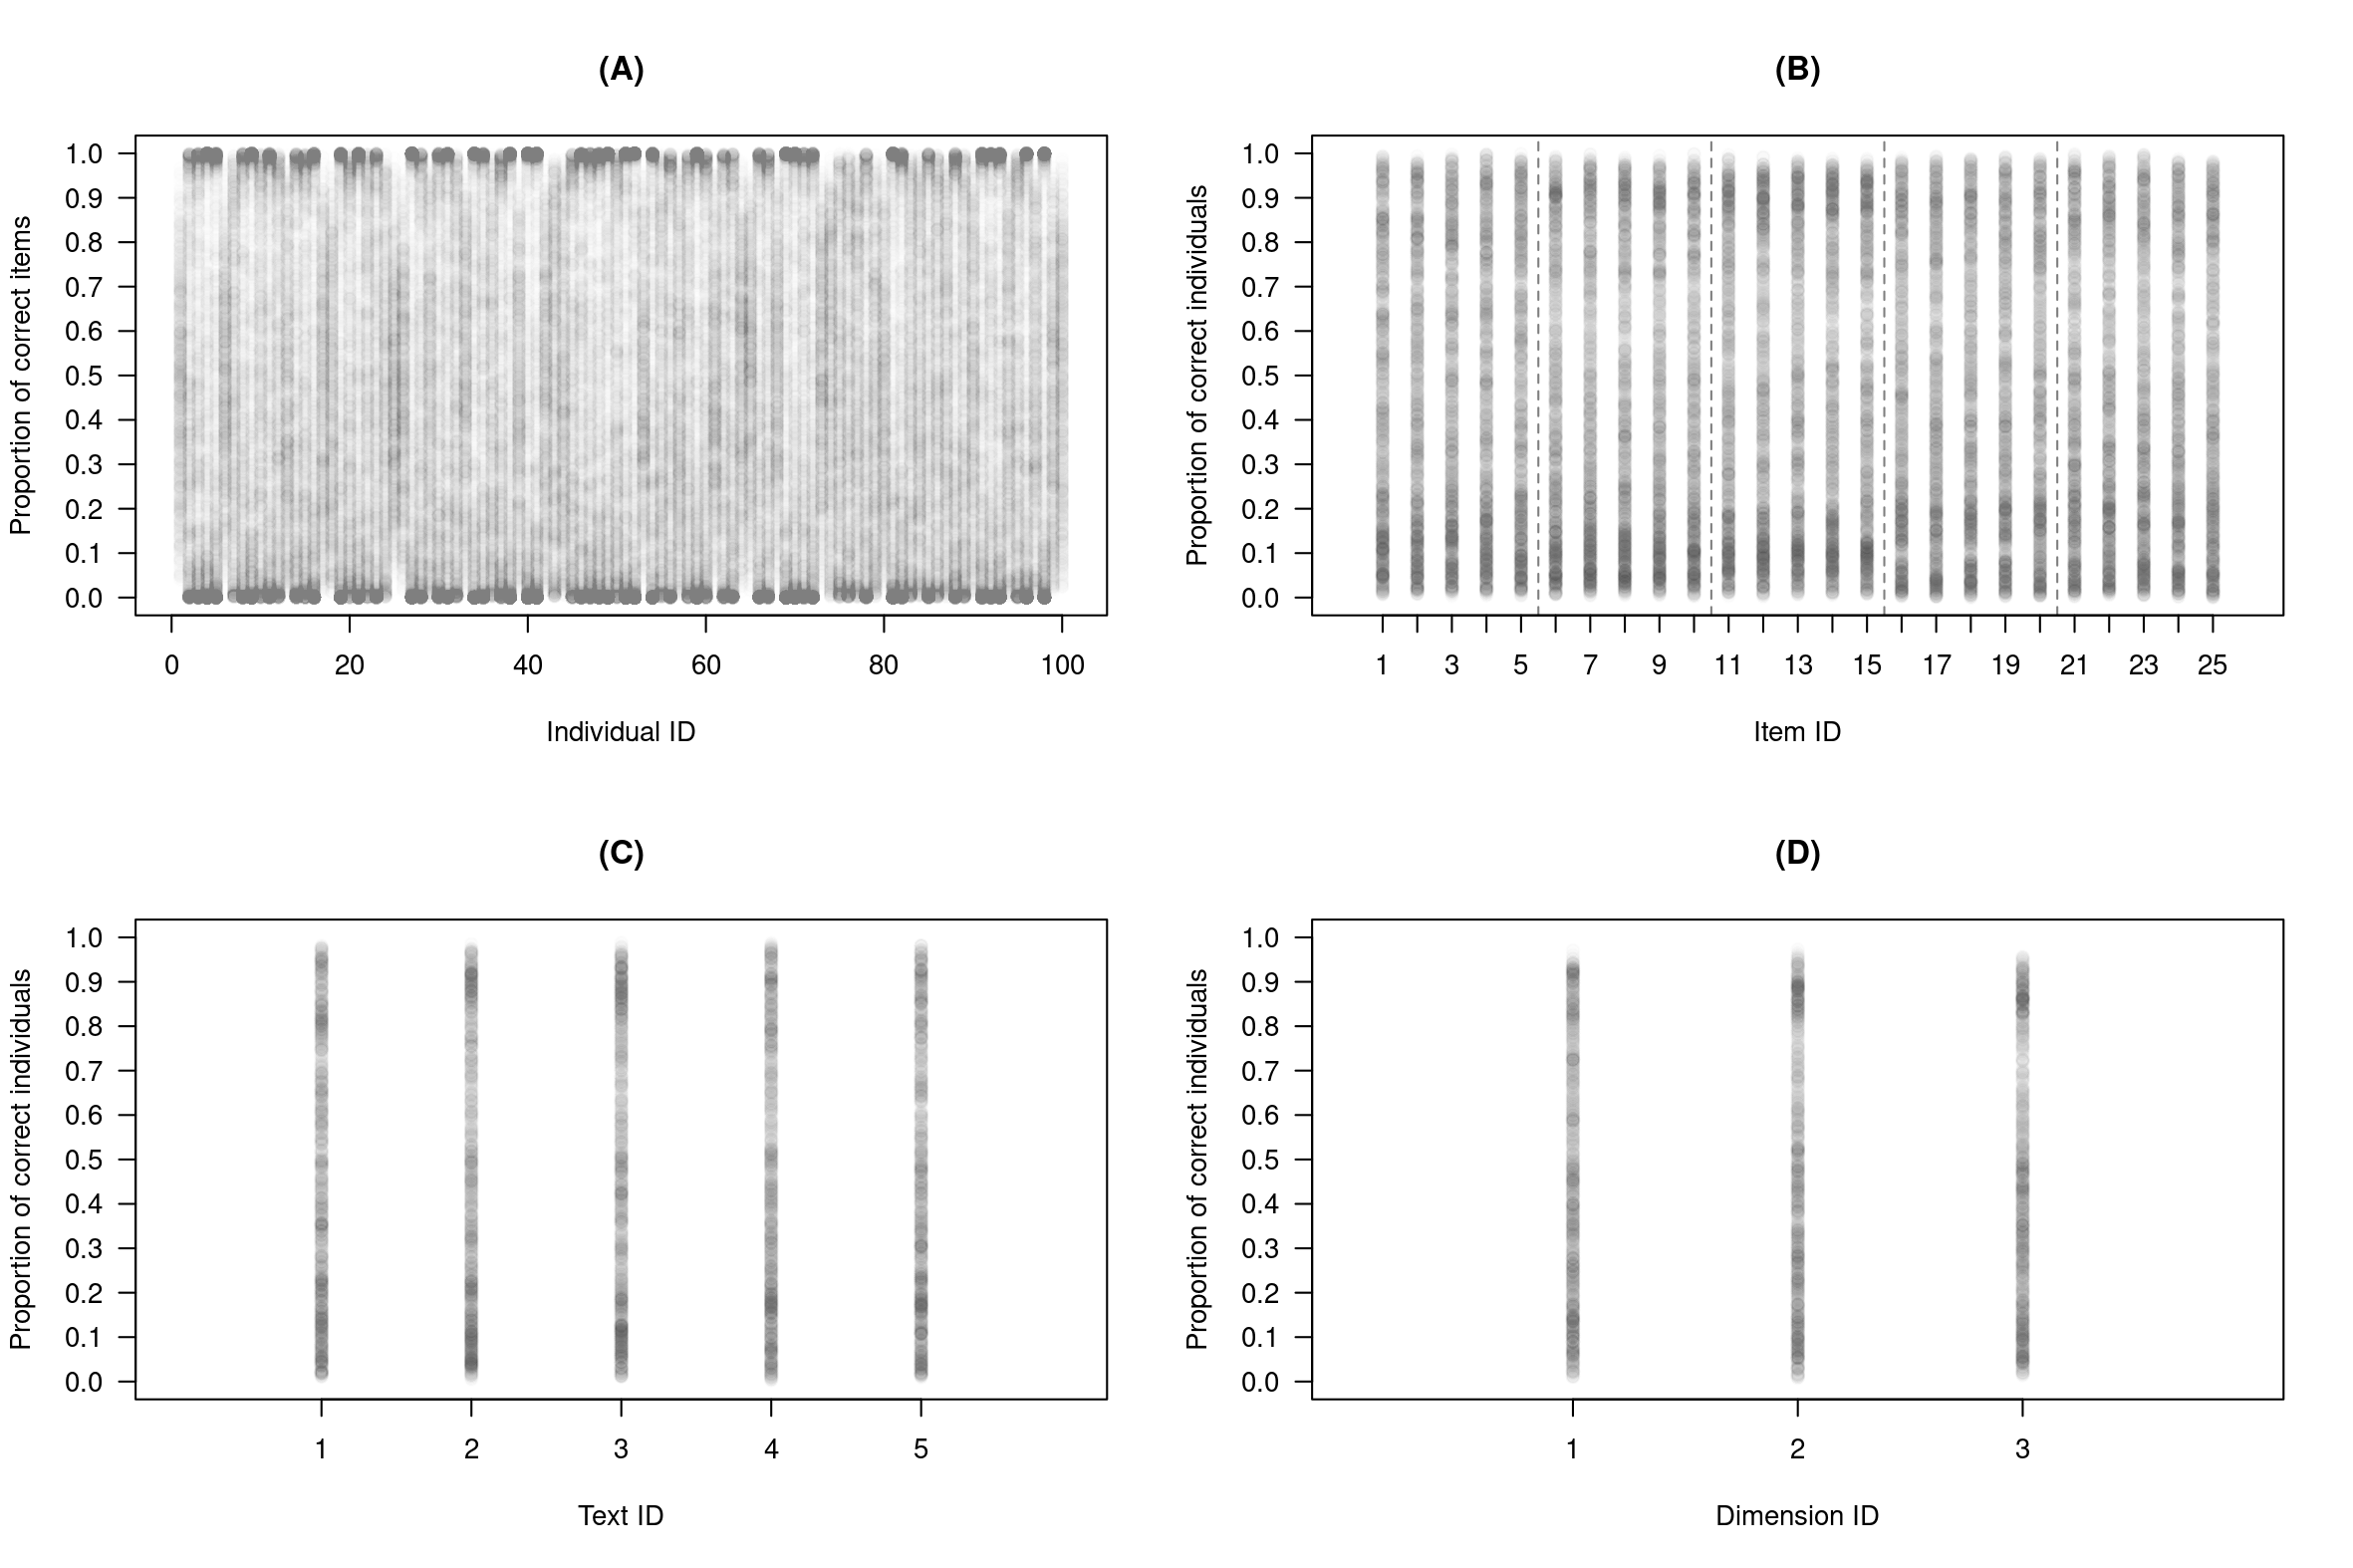
\includegraphics[width=1\linewidth]{FOLV_HitRate1}
	%
	\caption[First-order latent variable model (FOLV). Hit rate per dimensions of interest.]%
	{First-order latent variable model (FOLV). Aggregated endorsement rate per: (A) individuals, (B) items, (C) text or passage, and (D) measured dimension.}
	\label{fig:FOLV_hitrate1}
\end{figure}

Figure \ref{fig:FOLV_ICC_prior} shows the ICC and IIF for the FOLV model, resulting from the assumptions integrated by the priors detailed in the previous section. From panel (A), we can notice the difficulty of the items match a wide range of the individuals' abilities (see multiple black solid lines). This means the model expect items' difficulties to be in any part of the continuous range of abilities, with no restriction. Furthermore, the priors allow the model to obtain information about individuals located in the full significant range of the abilities, as seen in panel (B) of the same figure. All of this just means that no unintended assumption has ``creep" into the model, at least from the IRT perspective. A similar result can be seen for the SOLV model (figure \ref{fig:SOLV_ICC_prior}, appendix).

Finally, from figure \ref{fig:FOLV_hitrate1} and \ref{fig:FOLV_hitrate2}, we notice that no unintended assumption has been translated to the outcome space of the FOLV model, either. Panel (A) from figure \ref{fig:FOLV_hitrate1} shows the individuals'  proportion, of correctly answered items, can be present in the full range of possibilities. Furthermore, panel (B) of the same figure shows the proportion of individuals endorsing an item, for any item, can also be present in the full range of possibilities. Lastly, panels (C) and (D) convey similar information aggregated by texts and dimensions. On the other hand, all panels in figure \ref{fig:FOLV_hitrate2} revealed the prior distributions did not force any apriori tendencies in the covariates. A similar result can be seen for the outcome space of the SOLV model (figures \ref{fig:SOLV_hitrate1} and \ref{fig:SOLV_hitrate2}, appendix).
%
\begin{figure}[h]
	\centering
	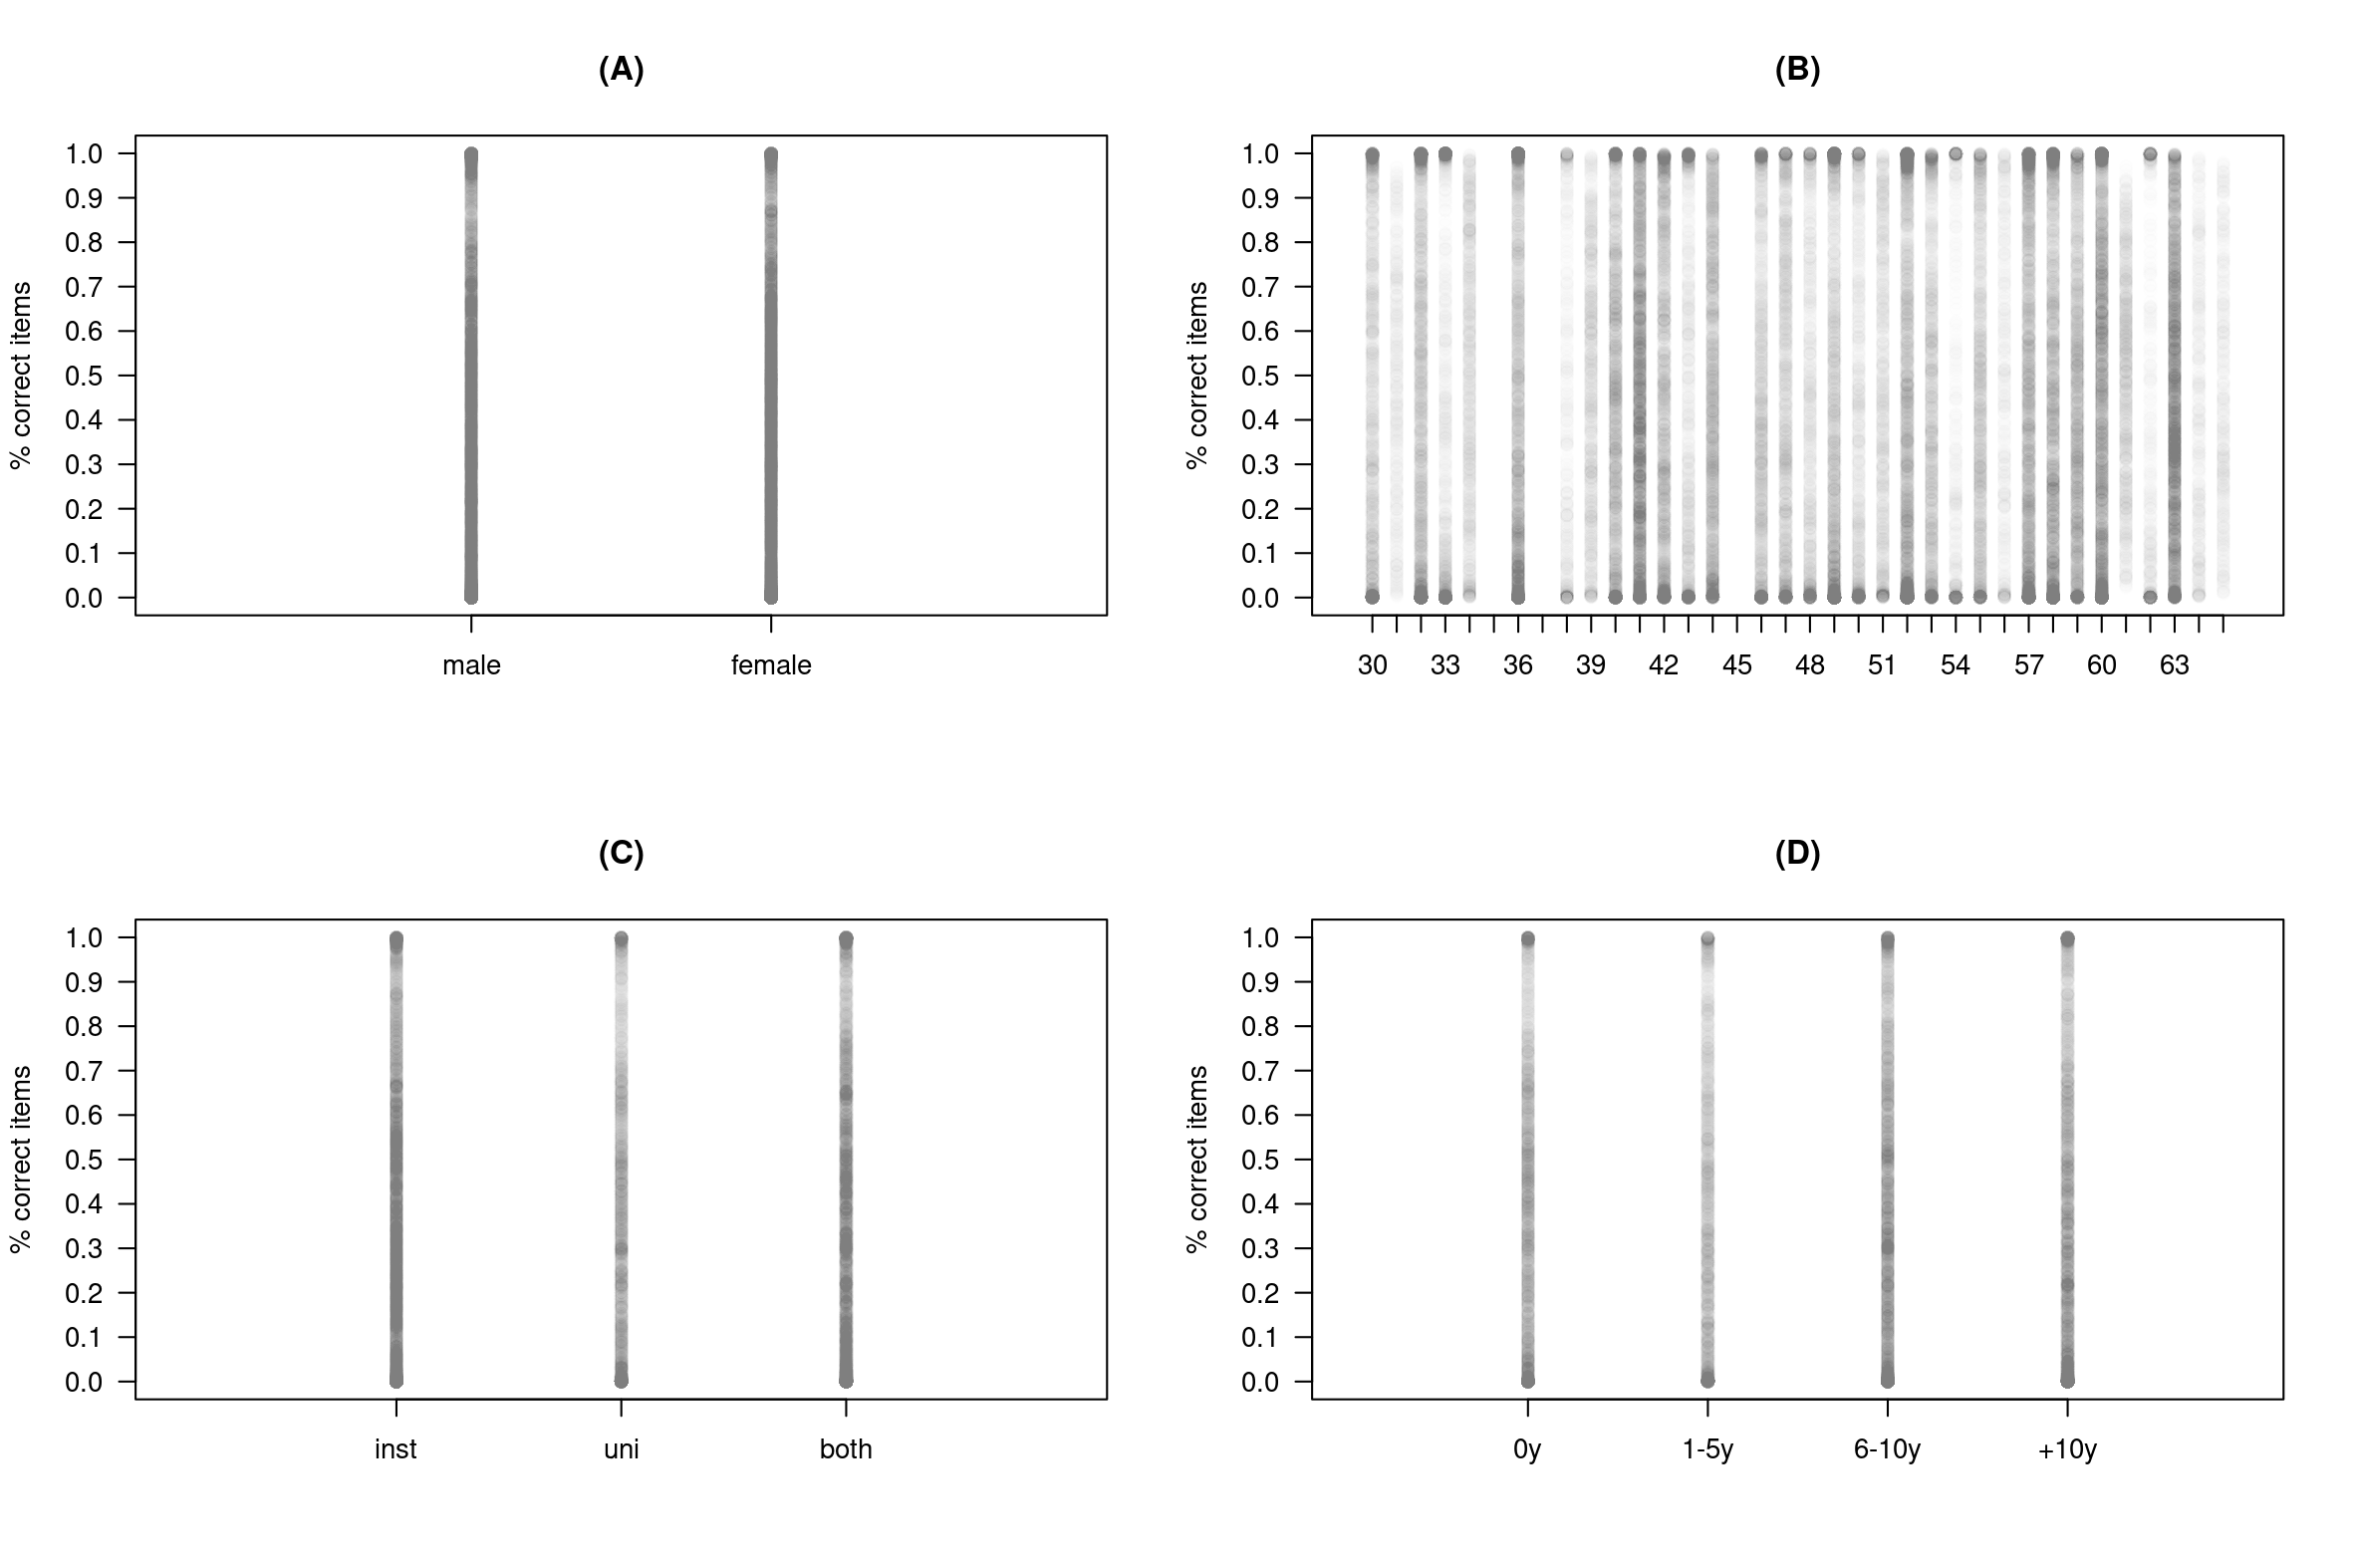
\includegraphics[width=1\linewidth]{FOLV_HitRate2}
	%
	\caption[First-order latent variable model (FOLV). Hit rate per simulated covariate.]%
	{First-order latent variable model (FOLV). Aggregated endorsement rate per simulated covariate: (A) gender, (B) age, (C) education, and (D) experience.}
	\label{fig:FOLV_hitrate2}
\end{figure}

%%%%%%%%%%%%%%%%%%%%%%%%%%%%%%%%%%%%%%%%%%%%%%%%%%%%%%%%%%%%%%%%%%%%%%%
%%%%%%%%%%%%%%%%%%%%%%%%%%%%%%%%%%%%%%%%%%%%%%%%%%%%%%%%%%%%%%%%%%%%%%%

\section{Results}

\subsection{Chain performance}

First, the CP and NCP chain performance for the texts' mean difficulties is reported in figures \ref{fig:FOLV_CE_chains1} and \ref{fig:FOLV_NC_chains1}, respectively. The figures correspond to replica number two of the FOLV model, with a simulated sample size of $100$. 

From the figures, one can easily notice the parameters under the CP did not show signs of achieving ergodicity. The chains showed a clear lack of stationarity and convergence (left panels). Moreover, the iterations did not explore the posterior distribution appropriately, as the several divergent transitions hinted, indicating a lack of good mixing, e.g. the top trace and trank plots show chains that slowly meander through specific areas of the posterior distribution. In addition, the ACF plots reveal the chain iterations were highly auto-correlated, another sign of bad mixing. All of this is further confirmed by panels (A) and (C) from figure \ref{fig:FOLV_stat1}, where we can see the CP has low effective samples sizes (\texttt{n\_eff}) and higher than appropriate \texttt{Rhat} values, compared to the NCP.

In contrast, the parameters from the NCP are closer to achieve ergodicity. The trace plots show chains that seem to be stationary and convergent. The trank plots show a rapid exploration of the full range of posterior distribution, with no divergent transitions on sight. And finally, the ACF plots showed the iterations were less auto-correlated. Again, this is further confirmed by figure \ref{fig:FOLV_stat1}, where the NCP show greater \texttt{n\_eff} and appropriate \texttt{Rhat} values, versus the CP.
%
\begin{figure}[H]
	\centering
	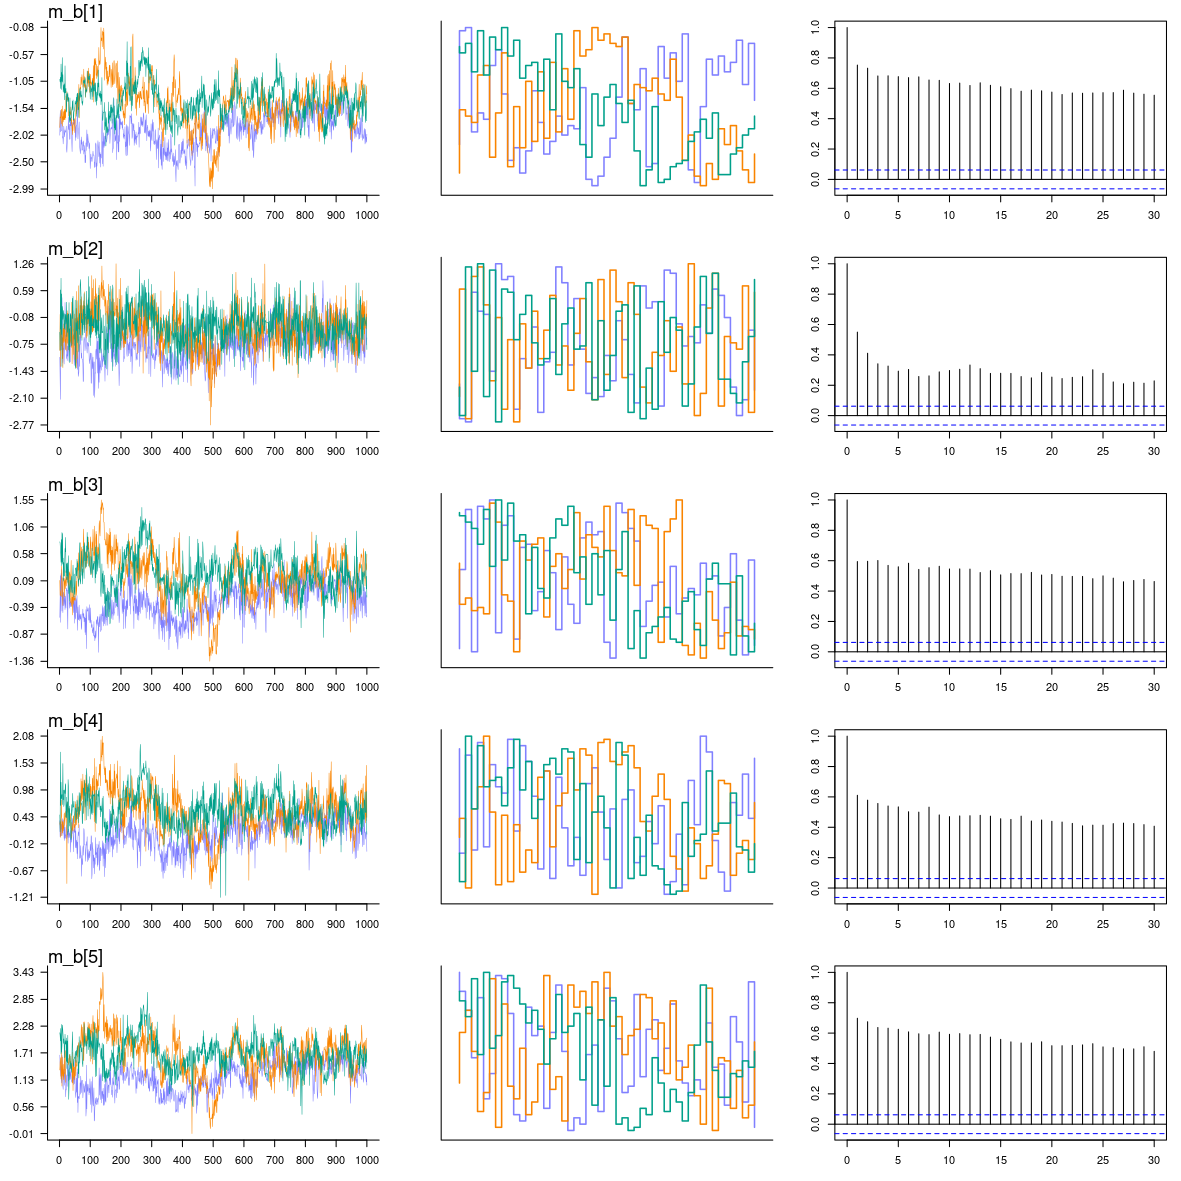
\includegraphics[width=1\linewidth]{FOLV_CE_J100_Ndata2_mb}
	%
	\caption[First-order latent variable model (FOLV). Sample size $100$, replica number $2$. Centered parametrization. Mean difficulty per text. Trace, trank and auto-correlation plots.]%
	{First-order latent variable model (FOLV). Sample size $100$, replica number $2$. Centered parametrization. Mean difficulty per text: (Left) trace plot, (Middle) trank plot, (Right) auto-correlation plot.}
	\label{fig:FOLV_CE_chains1}
\end{figure}

On the other hand, figures \ref{fig:FOLV_CE_chains2} and \ref{fig:FOLV_NC_chains2} (appendix) show the the CP and NCP trace, trank, and ACF plots for the the difficulties' deviations of the texts. At a simple glance, the plots seem to indicate that both parametrizations achieve a similar level of ergodicity. However, from panels (A) and (C) in figure \ref{fig:FOLV_stat1}, we can notice that while both parametrization show chains with \texttt{Rhat}$<1.05$, for some parameters, the CP has lower effective sample sizes than the NCP counterpart. The latter just indicates the NCP has less auto-correlated chains, and therefore a bit better mixing.
%
\begin{figure}[H]
	\centering
	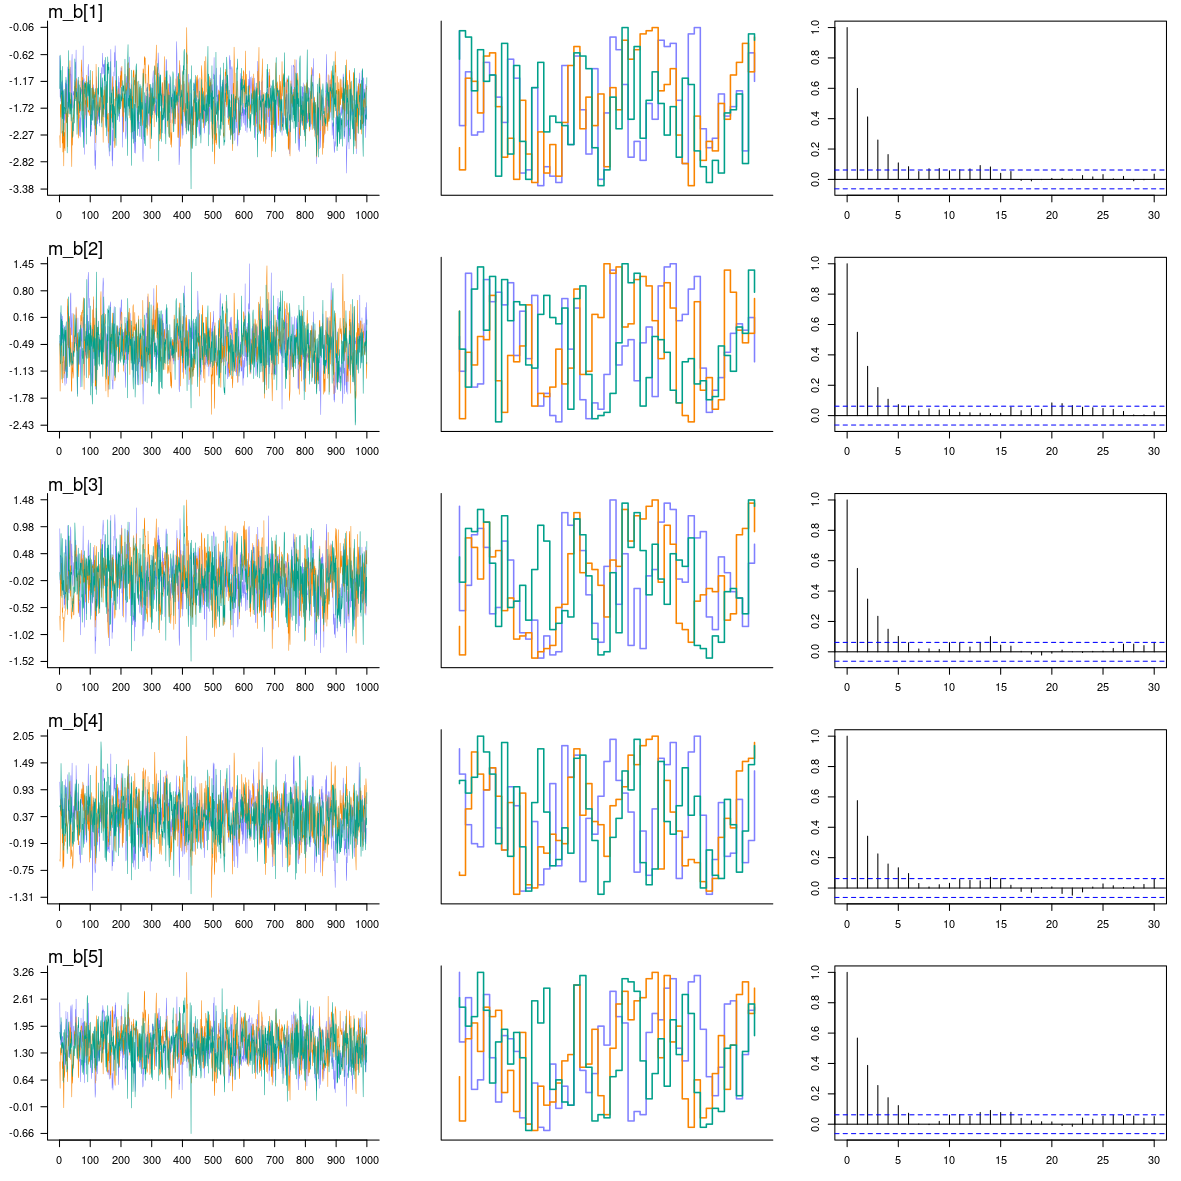
\includegraphics[width=1\linewidth]{FOLV_NC_J100_Ndata2_mb}
	%
	\caption[First-Order latent variable model (FOLV). Sample size $100$, replica number $2$. Non-centered parametrization. Mean difficulty per text. Trace, trank and auto-correlation plots.]%
	{First-Order latent variable model (FOLV). Sample size $100$, replica number $2$. Non-centered parametrization. Mean difficulty per text: (Left) trace plot, (Middle) trank plot, (Right) auto-correlation plot.}
	\label{fig:FOLV_NC_chains1}
\end{figure}

Furthermore, figures \ref{fig:FOLV_CE_chains3} and \ref{fig:FOLV_NC_chains3} (appendix) show the chain performance for the CP and NCP item difficulties. The trace, trank and ACF plots show a similar pattern as the one outlined for the difficulty of the texts, albeit more extreme. The CP chains did not achieved stationarity, convergence, nor good mixing; whereas the NCP does. This is further confirmed by panels (B) and (D) of figure \ref{fig:FOLV_stat1}, where one can see observe the NCP has significantly higher effective sample sizes and \texttt{Rhat}$<1.05$, in contrast to the CP.

Second, the CP chain performance for the reading comprehension sub-dimensions are reported in figures \ref{fig:FOLV_CE_chains4}, \ref{fig:FOLV_CE_chains5}, \ref{fig:FOLV_CE_chains6} (appendix). The figures correspond to several replicas of the FOLV model, with a simulated sample size of $100$. Similar to the preceding texts' difficulties, the chains also showed a lack of ergodicity, e.g. the left panels of figure \ref{fig:FOLV_CE_chains6} show chains that did not explore the posterior distribution appropriately (see straight lines in the trace plots). This is further confirmed by panels (A) through (D) in figure \ref{fig:FOLV_stat3}, where the CP has low effective sample sizes, while an important proportion of the parameters is above the recommended \texttt{Rhat} threshold. In contrast, the NCP chains for the sub-dimensions achieve ergodicity, as it is shown in figures \ref{fig:FOLV_NC_chains4}, \ref{fig:FOLV_NC_chains5}, \ref{fig:FOLV_NC_chains6}, and confirmed by the \texttt{n\_eff} and \texttt{Rhat} values in figure \ref{fig:FOLV_stat3}.
%
\begin{figure}[H]
	\centering
	\begin{subfigure}
		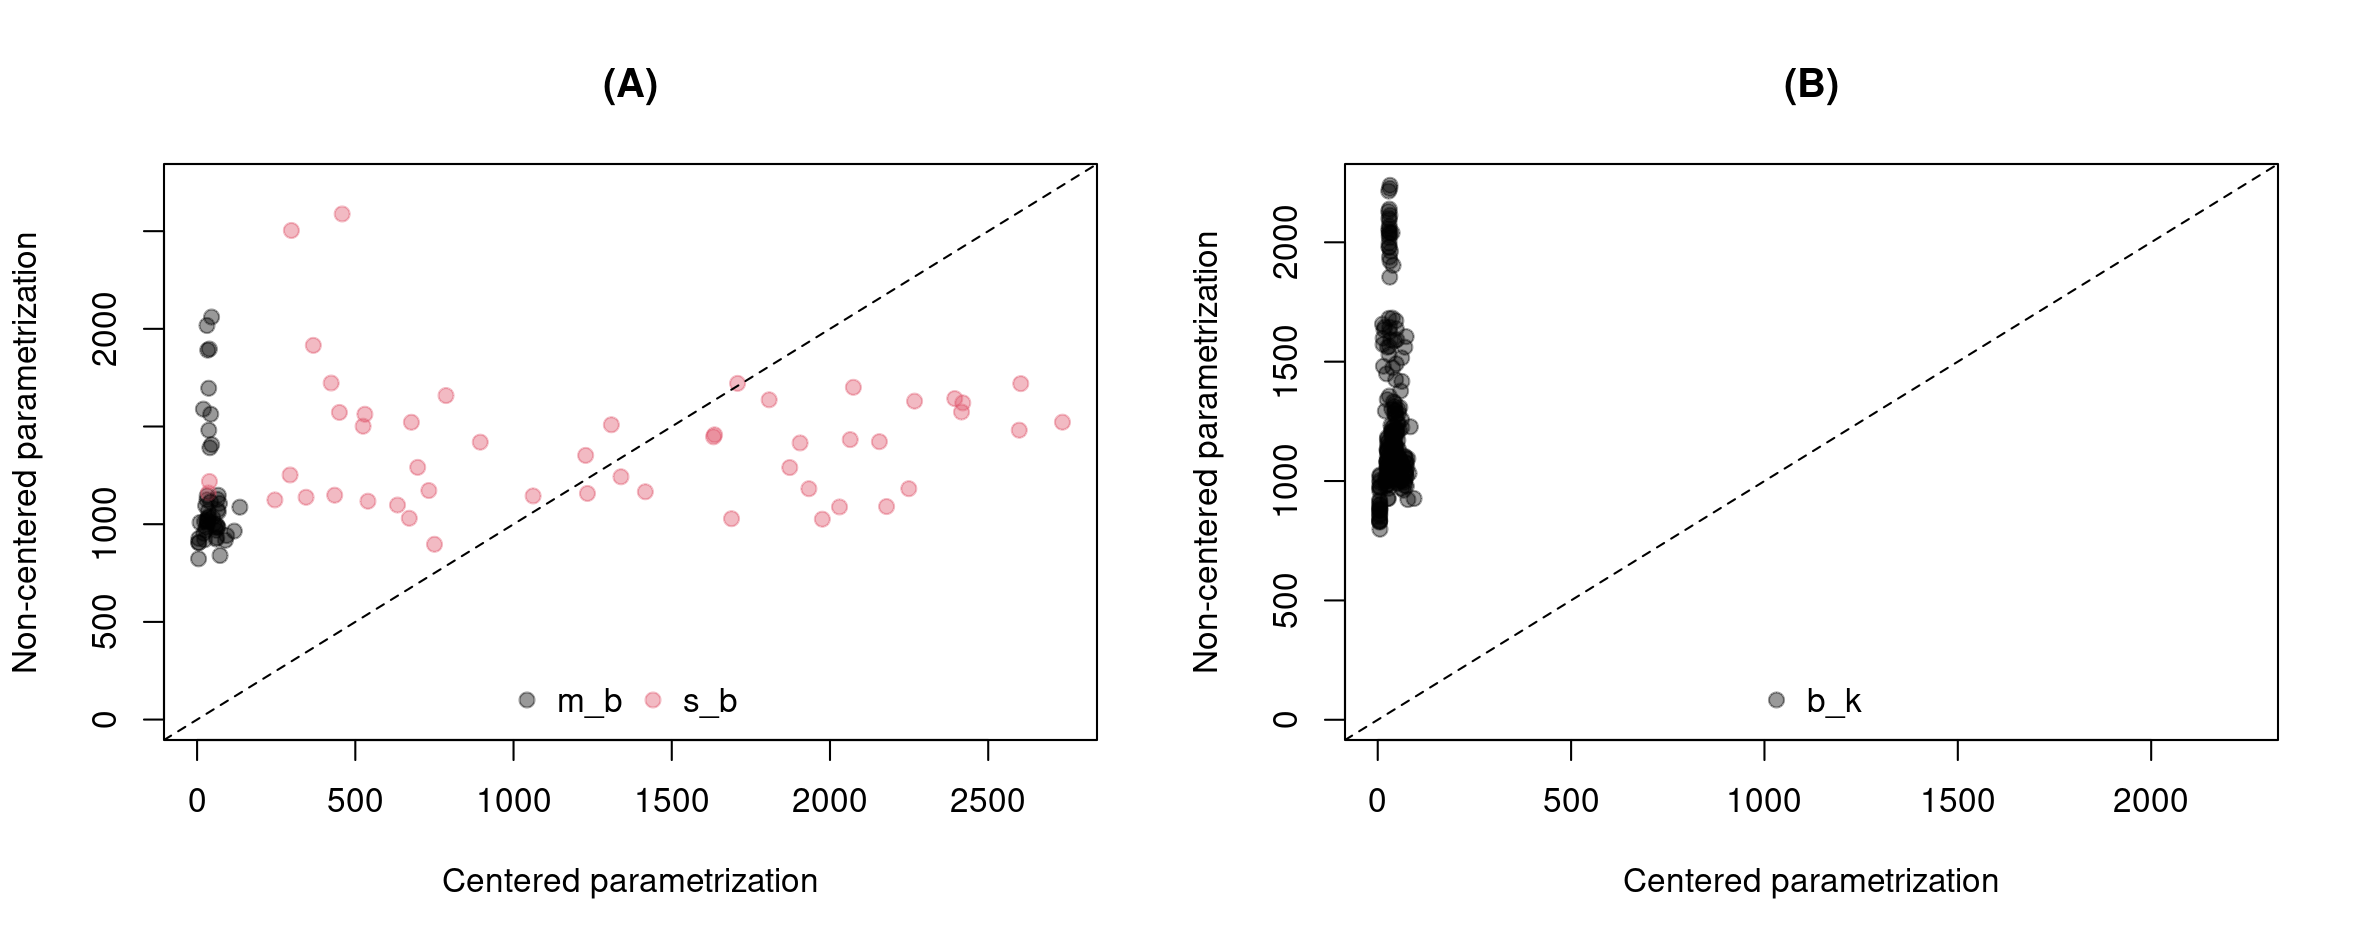
\includegraphics[width=1\linewidth]{FOLV_100_neff1}
	\end{subfigure}
	%
	\begin{subfigure}
		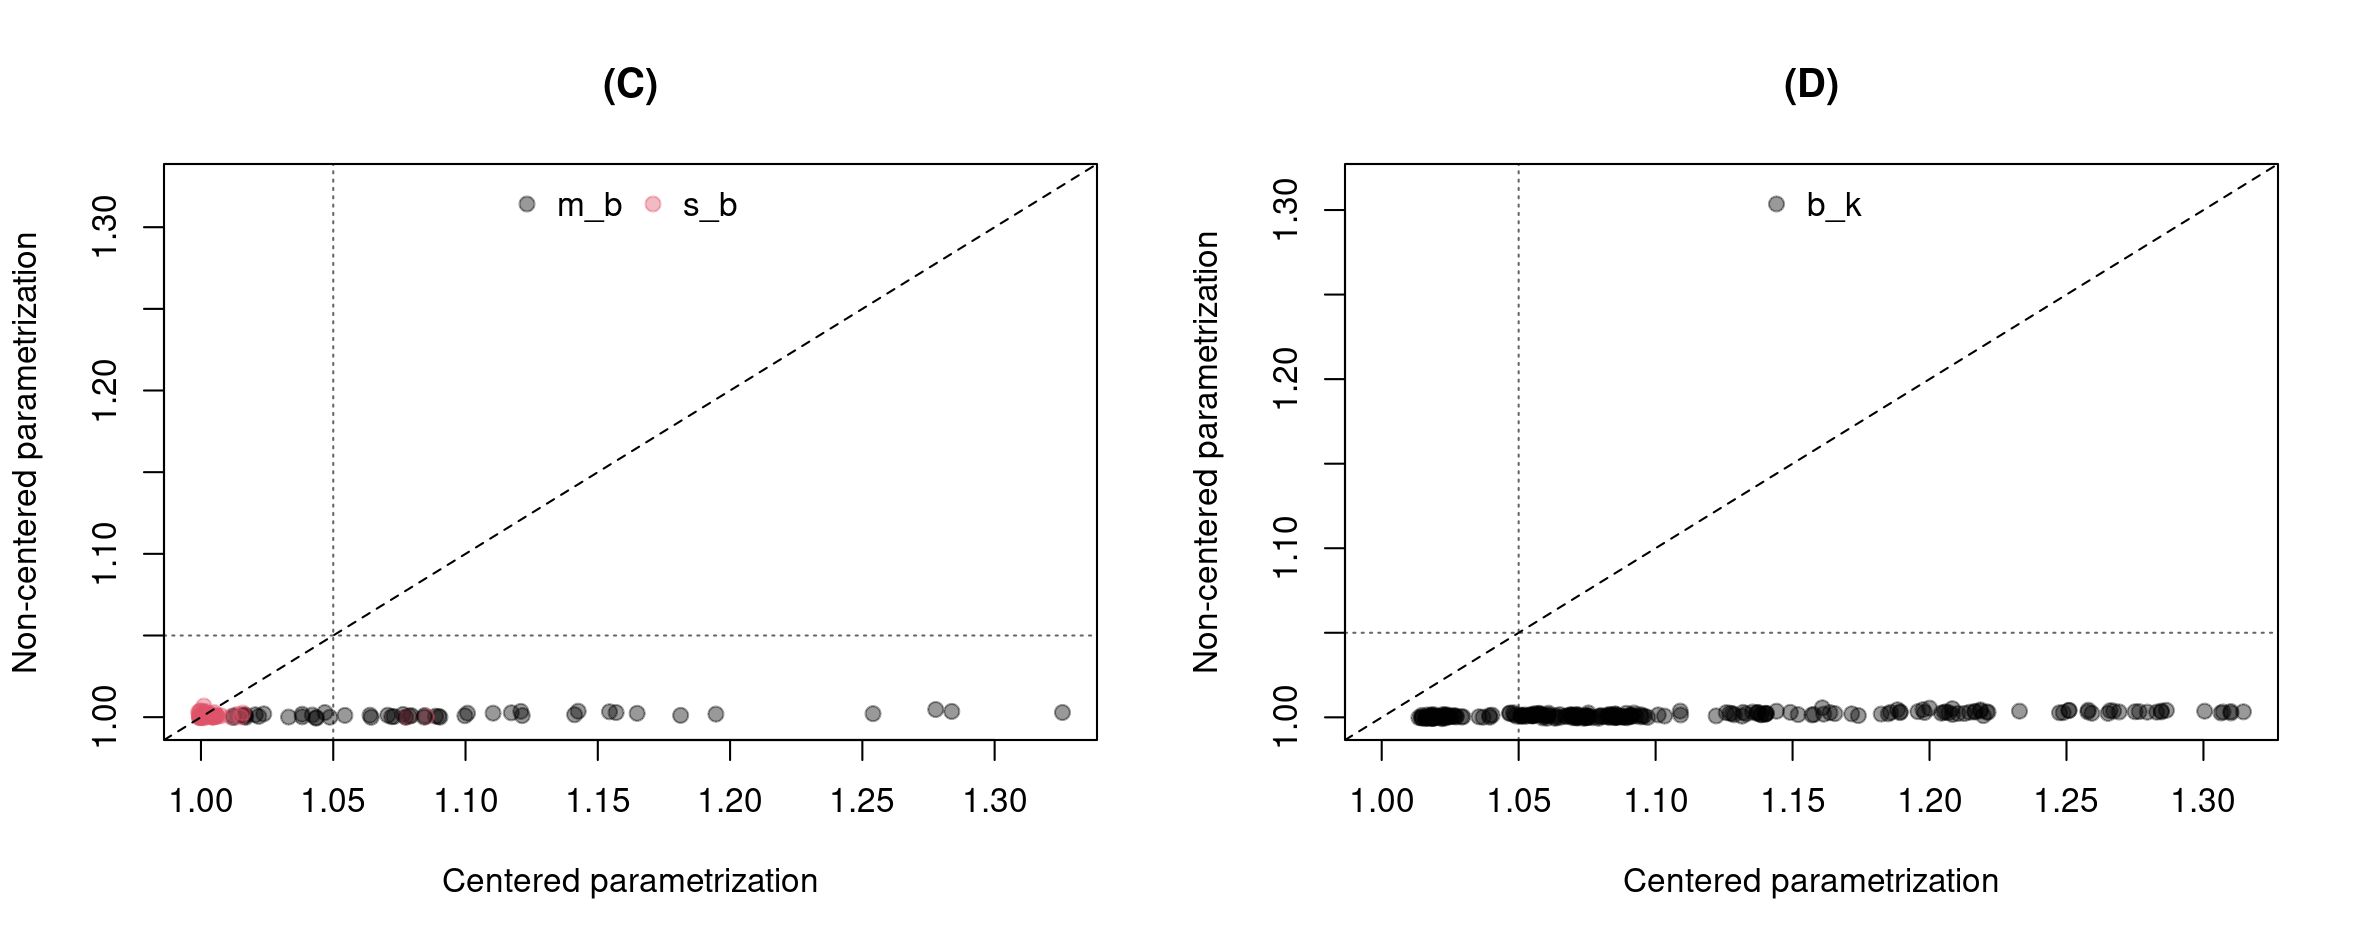
\includegraphics[width=1\linewidth]{FOLV_100_Rhat1}
	\end{subfigure}
	%
	\caption[First-order latent variable model (FOLV). Sample size $100$, all replicas. CP and NCP comparison plot.]%
	{First-order latent variable model (FOLV). Sample size $100$, all replicas. CP and NCP comparison plot. (A) \texttt{n\_eff} for texts' mean difficulty and standard deviation of difficulty. (B) \texttt{n\_eff} for items's difficulties. (C) \texttt{Rhat} for texts' mean difficulty and standard deviation of difficulty. (D) \texttt{Rhat} for items's difficulties. Diagonal discontinuous line describes equality between CP and NCP. Vertical and horizontal discontinuous lines is set at \texttt{Rhat}$=1.05$. }
	\label{fig:FOLV_stat1}
\end{figure}

Third, similar visualizations for the CP and NCP regression parameters are shown in appendix figures \ref{fig:FOLV_CE_chains7} and \ref{fig:FOLV_NC_chains7}. By a careful inspection of the CP trace plots, one can notice we still have chains that are ``stuck" in specific part of the posterior distribution (see green lines). As a result, the CP registered lower effective samples sizes than the NCP, as figure \ref{fig:FOLV_stat2} confirms. However, neither of those things prevented the CP achieving convergence, as the \texttt{Rhat} in the same figure confirms. In contrast, the NCP parameters seem to achieve stationarity, convergence, and good mixing without any issues, with higher effective sample sizes and \texttt{Rhat} values close to one.

Lastly, the performance assessment plots for the sub-dimensions' correlations of the FOLV model are shown in appendix figures \ref{fig:FOLV_CE_chains8} and \ref{fig:FOLV_NC_chains8}. In both parametrizations, we observe the correlations seem to achieve stationarity and convergence. However, it also seems they do not manage to make a proper investigation of the posterior. This is further confirmed by panels (B) and (D) from figure \ref{fig:FOLV_stat2}, where we see observe the parameters' chains remain below the \texttt{Rhat} recommended threshold, indicating convergence; although, the effective sample sizes were low, indicating highly auto-correlated iterations.

So far we have only compared the CP and NCP performance of the FOLV model, for specific replicas, and a simulated sample size of $100$. However, after the inspection of the trace, trank, ACF and comparison plots\footnote{To inspect the remaining trace, trank, ACF, and comparison plots follow the github accompanying page detailed in Appendix \ref{sub_sect:chain_performance}.}, we notice the preceding patterns of stationarity, convergence and mixing extends to all replicas, simulated sample sizes and parametrizations of the FOLV model. Furthermore, the aforementioned patterns were also observed in a similar parameter set the SOLV shares with the FOLV model. 

For the remaining parameters in the SOLV model, that is, the loadings and reading comprehension higher-order latent variables, we continue observing the same recurring patterns. Appendix figures \ref{fig:SOLV_CE_chains1} and \ref{fig:SOLV_NC_chains1} show the NCP loadings have chains that seem slightly more stationary, convergent, and well mixed than its CP counterpart. This is further confirmed by panels (B) and (D) from figure \ref{fig:SOLV_stat1}. In a similar fashion, figures \ref{fig:SOLV_CE_chains3} and \ref{fig:SOLV_NC_chains3} show the higher-order latent variable is significantly more ergodic under the NCP than the CP. Figure \ref{fig:SOLV_stat2} confirms the hypothesis, by showing it has larger effective sample sizes, with \texttt{Rhat} values always close to one.

Finally, panel (A) of figure \ref{fig:SOLV_stat3} show the pattern of ergodicity for the regression parameters is slightly improved under the SOLV model. The chains show larger effective sample sizes under the NCP versus the CP, indicating less correlation among the iterations, and therefore, better mixing. Ultimately, the patterns for this set of parameters was also consistent across replicas and simulated sample sizes.

\begin{comment}
The result appear to be sensible because of two factors, (i) as not only the different sub-dimensions are , but also beacuse the SOLV model was the data generating model.
\end{comment}

Consequently, all of the above just show the NCP largely improved the performance of the MCMC chains under our implementation, for all models and almost all of the parameters. It is important to point out, the result did not extend to the sub-dimensions' correlation parameters, where no large difference in performance was observed between the CP and NCP. On this matter, the issue was not related to a lack of identification of said parameters, as we were careful to ensure the fulfillment of this requirement (see next section for more evidence).

%%%%%%%%%%%%%%%%%%%%%%%%%%%%%%%%%%%%%%%%%%%%%%%%%%%%%%%%%%%%%%%%%%%%%%%

\subsection{Recovery capacity}

Figures \ref{fig:FOLV_CE_recovery1} and \ref{fig:FOLV_NC_recovery1} show the CP and NCP recovery of the regression, contrast, and correlation parameters for the first replica of the FOLV model, with a sample size of $100$. From both figures we notice the regression and contrast parameters were estimated appropriately. The true values were located within the compatibility interval of the estimates. Moreover, no remarkable difference is observed between the CP and NCP implementations. This result extends across all replicas and sample sizes, as the recovery plots\footnote{To inspect the remaining recovery plots follow the github accompanying page detailed in Appendix \ref{sub_sect:recovery}.} confirm. Furthermore, table \ref{tab:FOLV_RMSE_regression} (appendix) reveal the $\text{RMSE}_{B}$ of the regression parameters under NCP were consistently lower than the CP counterpart, but the differences were negligible. In a similar fashion, table \ref{tab:FOLV_RMSE_contrasts} show a similar pattern in the contrast parameters, between the CP and NCP; however, we also observe the contrasts were recovered with better precision with larger sample sizes, no matter the parametrization.
%
\begin{figure}[H]
	\centering
	\begin{subfigure}
		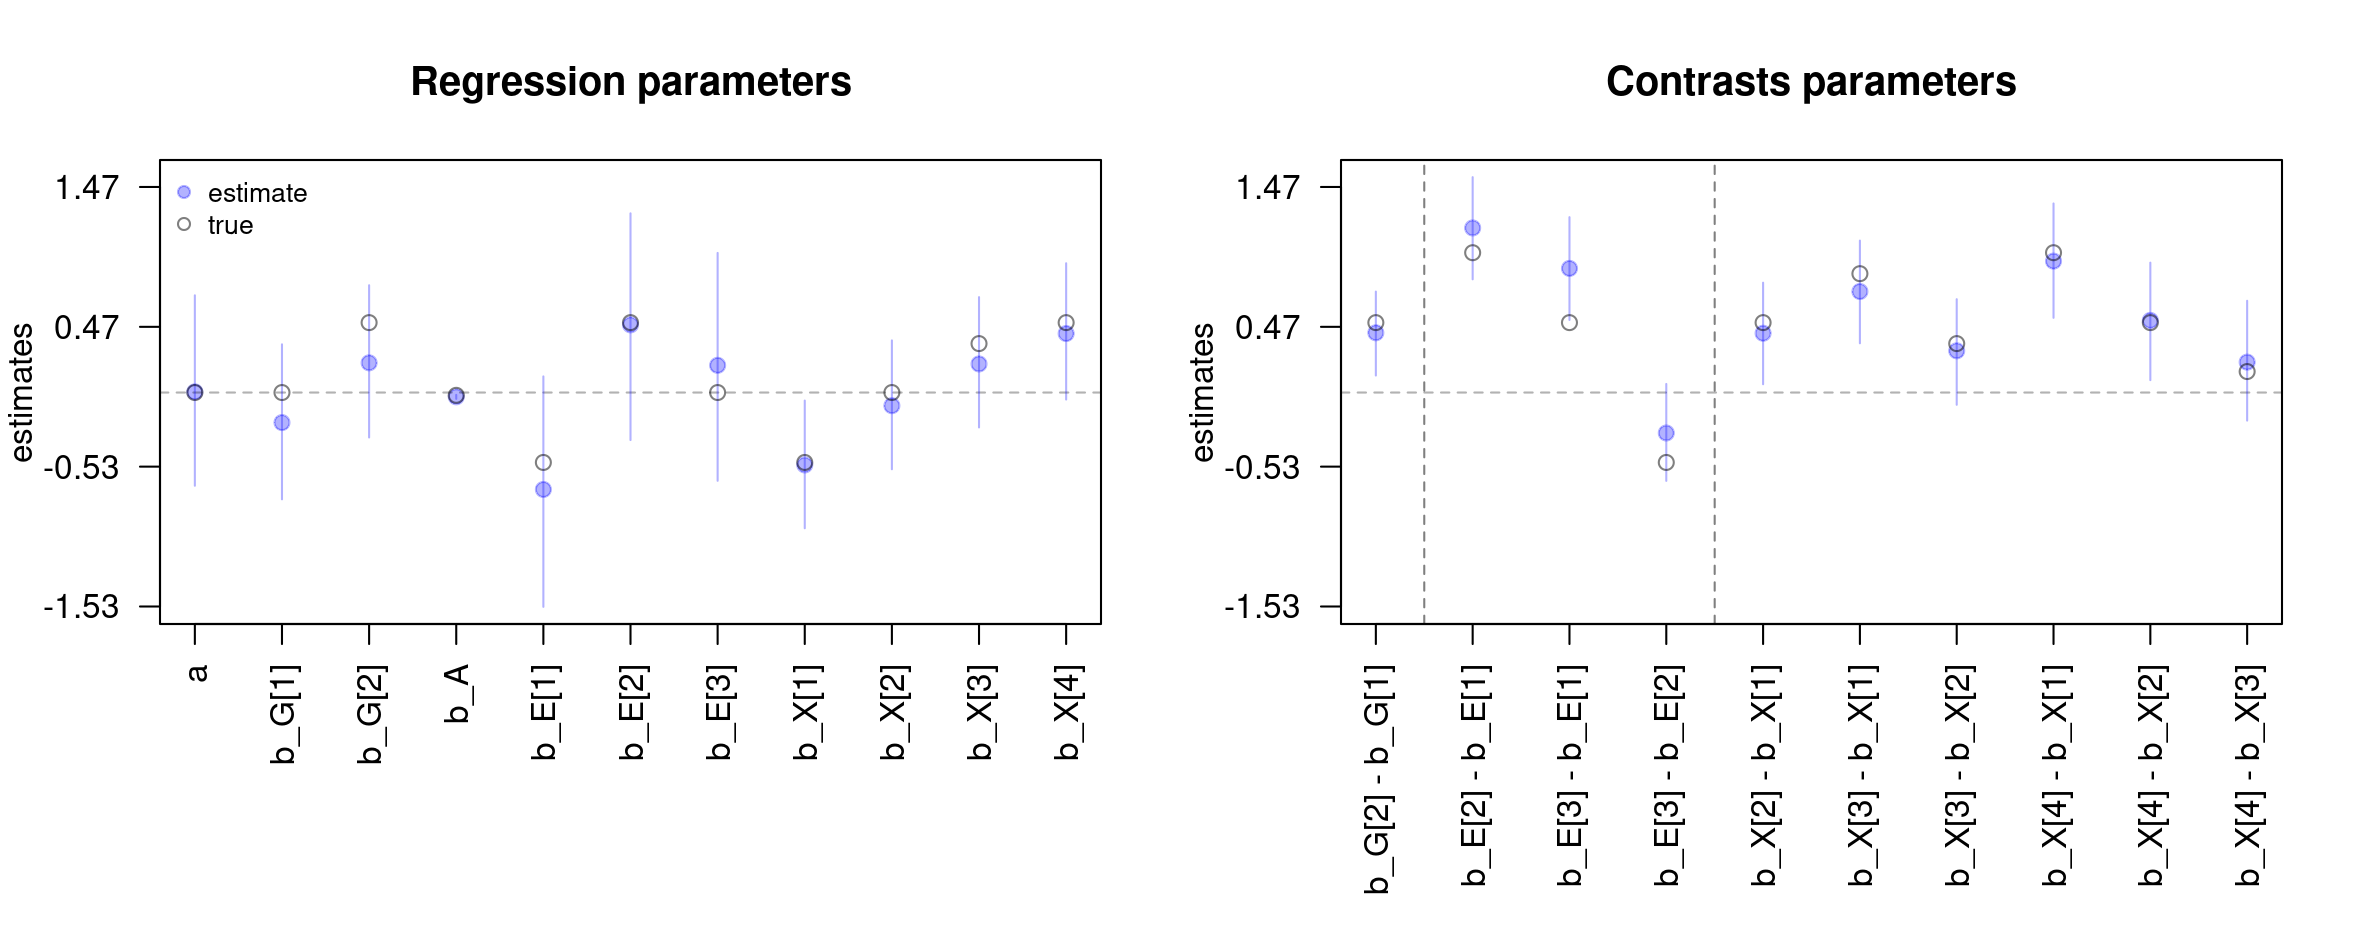
\includegraphics[width=1\linewidth]{FOLV_CE_J100_Ndata1_regression}
	\end{subfigure}
	%
	\begin{subfigure}
		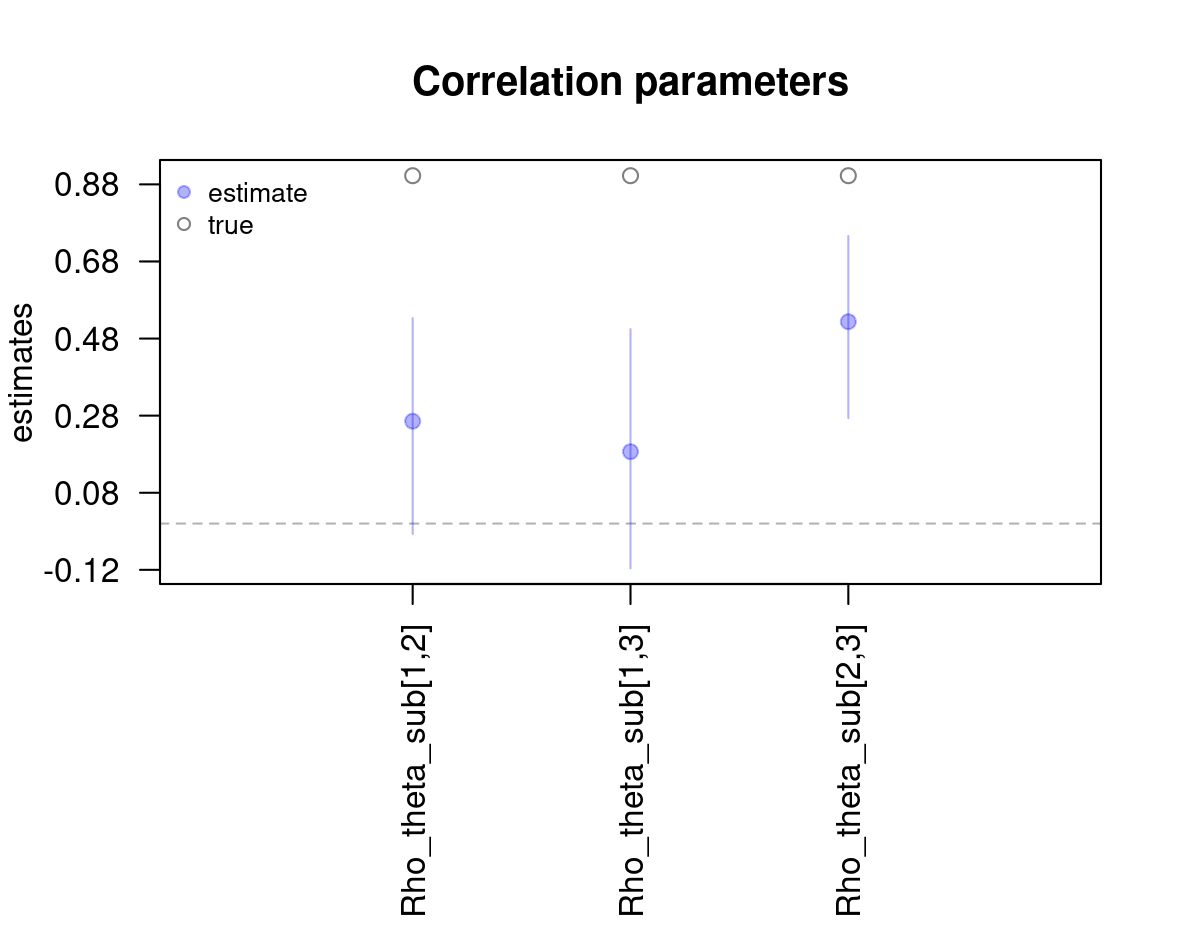
\includegraphics[width=0.5\linewidth]{FOLV_CE_J100_Ndata1_corr}
	\end{subfigure}
	%
	\caption[First-order latent variable model (FOLV). Centered parametrization. Sample size $100$, replica $1$. Regression, contrast, and correlation parameters.]%
	{First-order latent variable model (FOLV). Centered parametrization. Sample size $100$, replica $1$. Regression, contrast, and correlation parameters. The ``true" correlation parameters were calculated using Wright's tracing rules, and corresponds to an approximate unconditional correlation.}
	\label{fig:FOLV_CE_recovery1}
\end{figure}

On the other hand, in the same figures, we notice the CP and NCP correlation parameters were estimated similarly far from the approximate unconditional correlations. The unconditional correlations were calculated using Wright's tracing rules \cite{Beaujean_2014} using the simulated loadings $\lambda^{(2)}_{d} = 0.95$, therefore, the approximate correlation was $0.95 \times 0.95 = 0.9025$. However, the comparison is misleading because the correlation parameters produced by the model were not unconditional. Recall the FOLV model used regression covariates to explain some of the variability in the sub-dimensions, therefore, the reported correlations are the residual correlations, after controlling for the aforementioned covariates. In that sense, we notice a non-negligible (and sometimes significant) amount of correlation remains present among the sub-dimensions, apparently due to the miss-specification of the model. Again, this behavior is consistent across replicas, and samples sizes, with no discernible difference among parametrizations (see table \ref{tab:FOLV_RMSE_corr}, appendix).
%
\begin{figure}[H]
	\centering
	\begin{subfigure}
		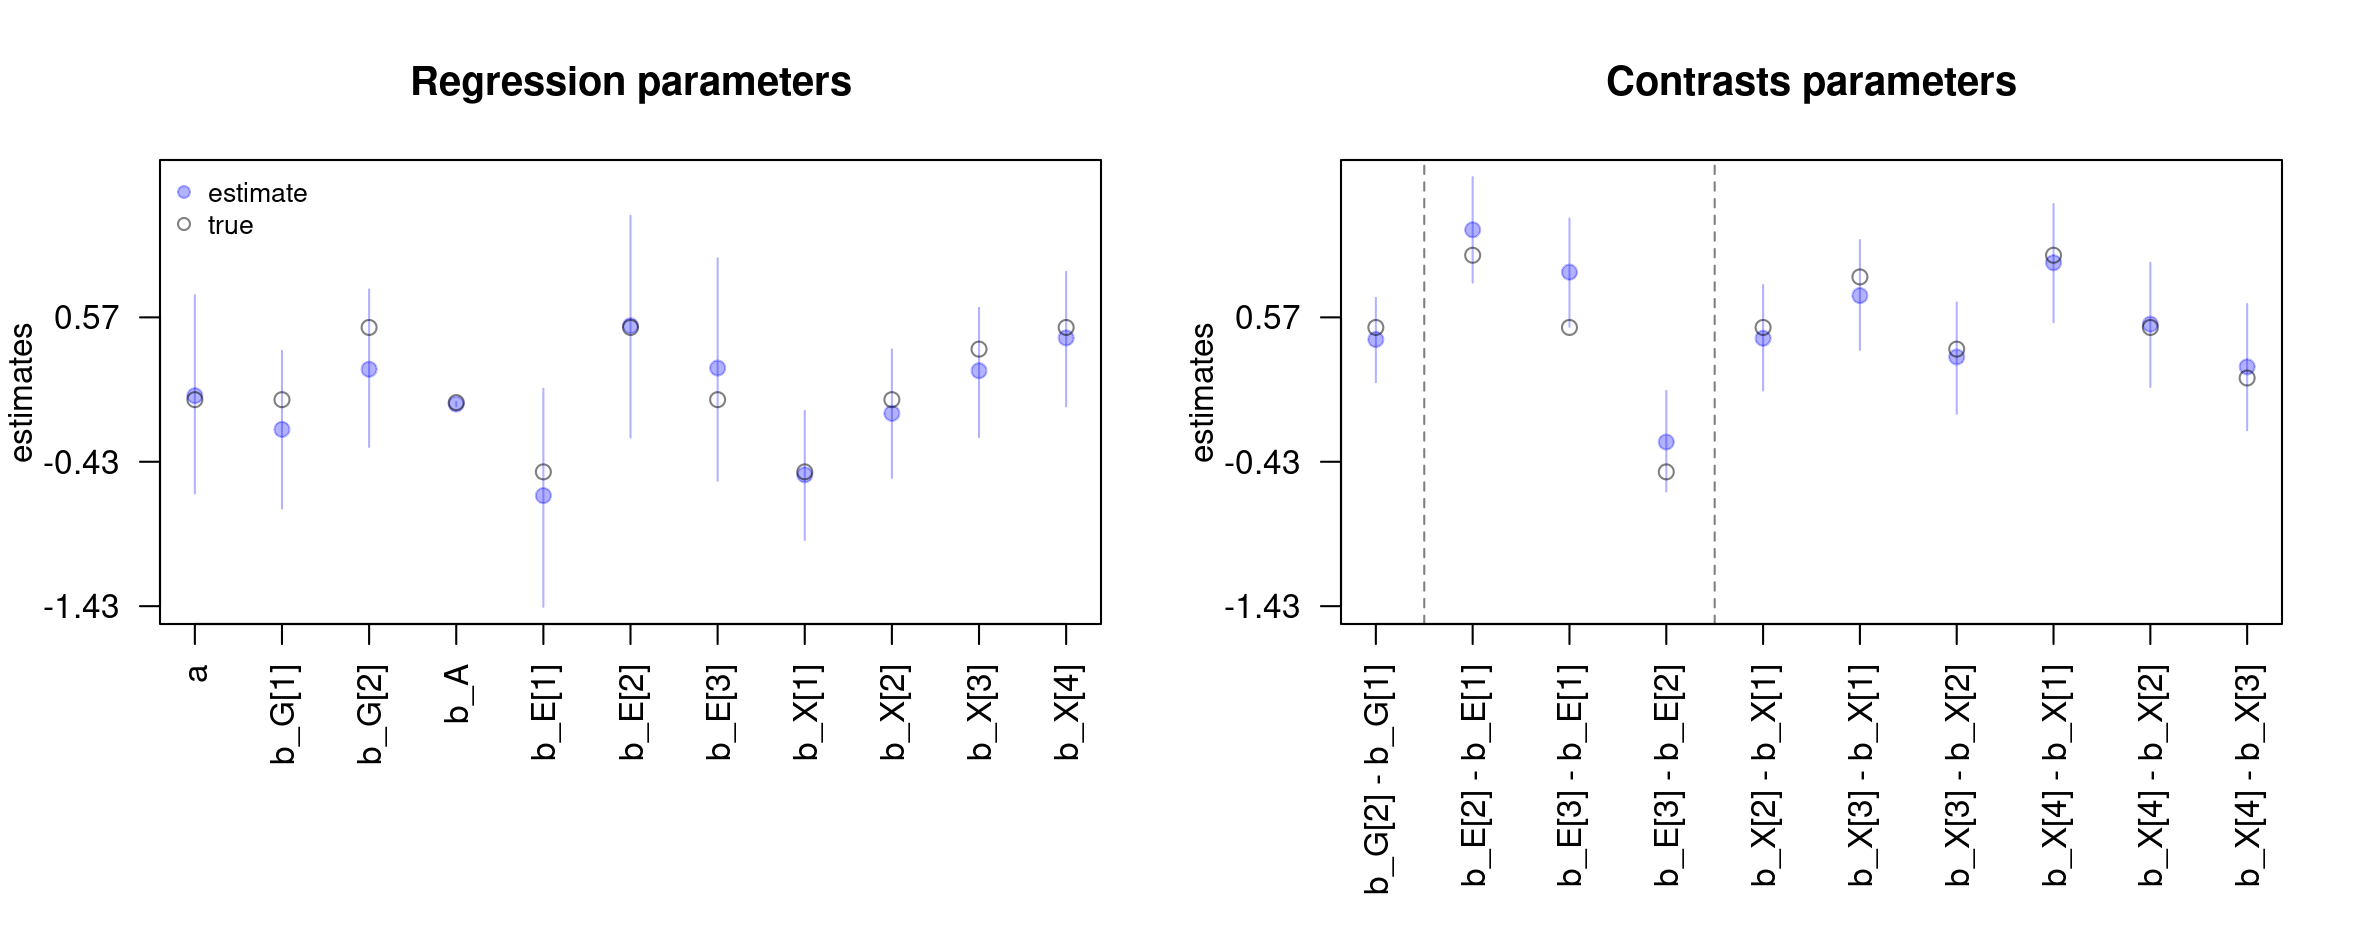
\includegraphics[width=1\linewidth]{FOLV_NC_J100_Ndata1_regression}
	\end{subfigure}
	%
	\begin{subfigure}
		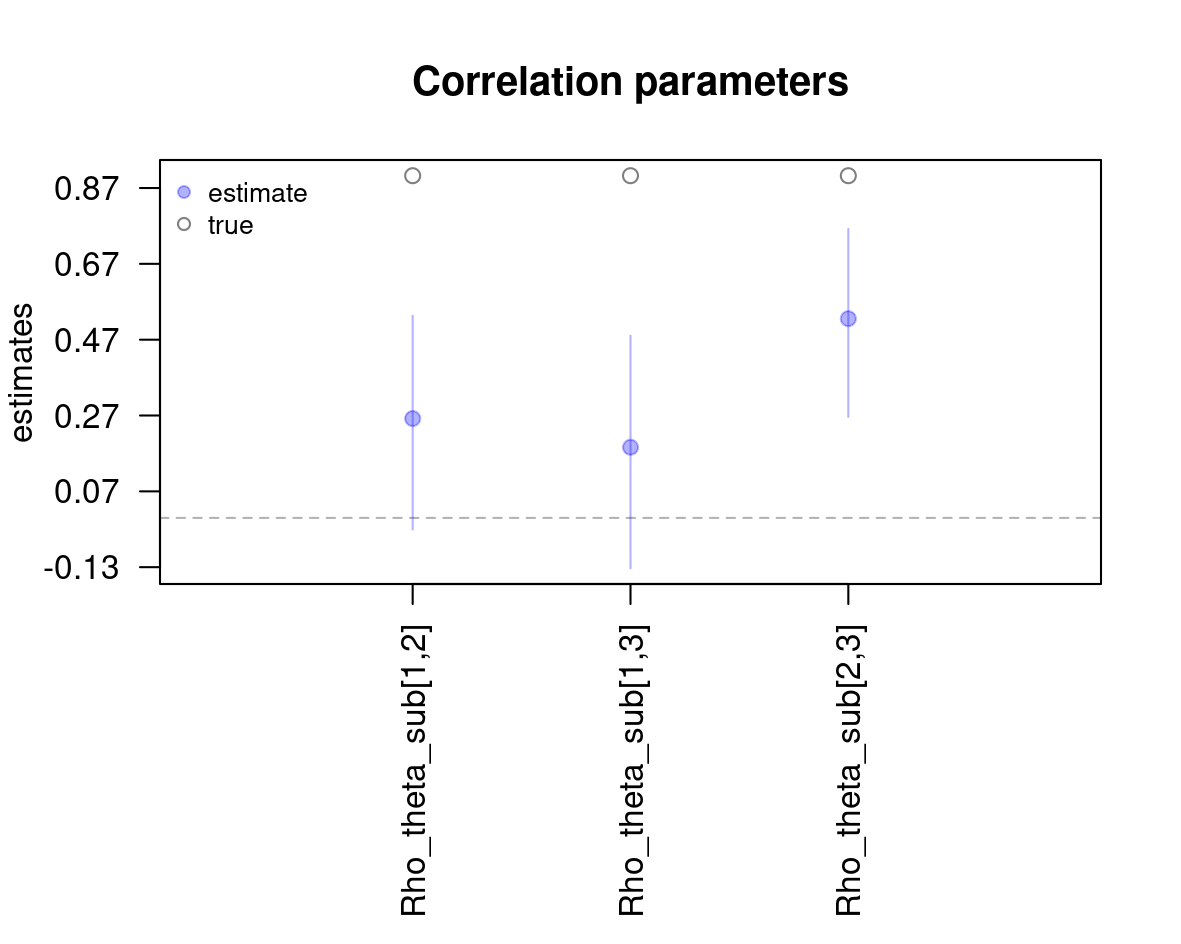
\includegraphics[width=0.5\linewidth]{FOLV_NC_J100_Ndata1_corr}
	\end{subfigure}
	%
	\caption[First-order latent variable model (FOLV). Non-centered parametrization. Sample size $100$, replica $1$. Regression, contrast, and correlation parameters.]%
	{First-order latent variable model (FOLV). Non-centered parametrization. Sample size $100$, replica $1$. Regression, contrast, and correlation parameters. The ``true" correlation parameters were calculated using Wright's tracing rules, and corresponds to an approximate unconditional correlation.}
	\label{fig:FOLV_NC_recovery1}
\end{figure}

Furthermore, figure \ref{fig:FOLV_recovery2} show the CP and NCP items, text, and text deviation difficulty estimates. As with the previous patterns of recovery, no remarkable difference was observed among the different parametrizations. On both scenarios, the true items and text difficulties were within the compatibility intervals of the bayesian implementation, while the text difficulties and deviations were estimated with greater precision. As in the previous estimates, the patterns were consistent across replicas, and samples sizes, with no discernible difference among parametrizations (see tables \ref{tab:FOLV_RMSE_texts_dev} and \ref{tab:FOLV_RMSE_items}, appendix).

A behavior somewhat similar is observed for the SOLV model. Figures \ref{fig:SOLV_CE_recovery1} and \ref{fig:SOLV_NC_recovery1} (appendix) show the CP and NCP regression, contrast, correlation and loading parameters. From the figures we notice the regression parameter were estimated equally well by both parametrizations. However, we notice in general, the model had a harder time to estimate the regression, contrast and correlation parameters, compared to the FOLV model. In the case of the regression parameters, table \ref{tab:SOLV_RMSE_regression} show the SOLV model had larger levels of errors for sample sizes of $500$. For the contrasts, on the other hand, table \ref{tab:SOLV_RMSE_contrasts} reveals the model estimated all parameters with higher error. This is particularly true for the contrast related to the education covariate. Moreover, one would think that, given the model is now correctly specified, the estimated correlations could be close to the true simulation parameters, but we would be wrong; and table \ref{tab:SOLV_RMSE_corr} hides this fact. From a careful inspection of the recovery plots\footnote{Not shown in the document. Refer to the corresponding github accompanying page detailed in Appendix \ref{sub_sect:recovery}.}, we can notice the SOLV model estimated non-negligible positive correlations for some of replicas with sample sizes greater than $100$. This just indicates that for larger sample sizes, some residual correlation remains present, even when the model considers a higher order latent variable. One explanation for this could be that the model severely underestimated the loadings. The true values for the parameters were not within any of the compatibility intervals (that is why we registered higher levels of $\text{RMSE}_{B}$ in table \ref{tab:SOLV_RMSE_loads}). Moreover, one could further argue that this is due to a lingering parameters' lack of identification, however, the evidence from the pairs plot\footnote{Same as previous footnote.} does not seem to support the hypothesis. The pairs plots show loadings and correlation with low levels of interdependence, contrary to the ``narrow ridge" pattern expected under the lack of identification hypothesis. Ultimately, in concordance with the FOLV model, these patterns of recovery were consistent across replicas, samples sizes, with no discernible difference between parametrizations.

Finally, appendix \ref{sub_sect:recovery} provides the FOLV and SOLV tables of the $\text{RMSE}_{B}$ for the latent individuals' dimensions. As with the preceding parameters, no discernible difference in the recovery capacity was observed between the CP and NCP. The results were consistent across replicas and sample sizes, as the several tables confirm. 

Nevertheless, it is surprising to observe the CP and NCP have a similar recovery capacity, as one could argue that in the case of simulation based estimation methods, like MCMC, the recovery capacity is highly tied to the performance of the procedure (conditional on the number of chosen iterations). The reader can recall from the previous section, that under the CP, multiple parameter chains fail to achieve ergodicity, therefore, jeopardizing our ability to make valid inferences about them. 

One explanation for this could be that both parametrizations achieved what is called a \textit{local convergence} \cite{Depaoli_2021}, that is, the chains appear to be stable in the range of the iterations (stability observed at least in the NCP). However, given the consistent results across replicas, the researcher is led to think that even with all the issues present under the CP, the chains managed to visit the posterior distribution in a way, that allowed the method to produce a proper estimation of the parameters. Moreover, we are also led to think, the preceding patterns of recovery capacity are the result of using the HMC algorithm with a higher rejection criteria (\texttt{adapt\_delta}$=0.99$) and weakly regularizing priors. The previous chapter has described the benefits of these factors separately, so it is sensible to assume that used in conjunction, they could benefit the posterior exploration, and therefore, the recovery capacity of the method. Further investigations manipulating these conditions could be of relative importance.


%%%%%%%%%%%%%%%%%%%%%%%%%%%%%%%%%%%%%%%%%%%%%%%%%%%%%%%%%%%%%%%%%%%%%%%

\subsection{Retrodictive accuracy}

Figure \ref{fig:FOLV_NC_hitrate_ind} shows the true, average, and marginal predicted proportions, on a random sample of individuals, of the fourth replica from the NCP FOLV model with a sample size of $100$. The plot also depicts the corresponding shrinkage and compatibility intervals. 

From the figure we notice the model manages to capture rather well the traits of the data, while avoiding its exact replication. We observe the true proportion of endorsed items, among individuals, are within the compatibility intervals of the average and marginal predictions, i.e. the true simulated values for the proportions are close to the predicted mean and outcomes produced by the model. However, we observe the average and marginal predictions show some level of shrinkage, that is, the estimates are ``pulled" towards the average true proportion across individuals, in greater or less quantity. This results from the complex pooling of information across individuals, items, texts and dimensions; that allows the model to negotiate between predicting all individuals with the average proportion (under-fitting) or predicting each individual by its own proportion (over-fitting). On the other hand, figure \ref{fig:FOLV_NC_hitrate_var} only confirms the model manages to capture the traits of the data, as the predicted proportions per individual and covariate combination, are replicated rather well. Similar results can be observed on the predictive accuracy of the model aggregated by dimensions, items, and texts, in figures \ref{fig:FOLV_NC_hitrate_items}, \ref{fig:FOLV_NC_hitrate_dim}, and \ref{fig:FOLV_NC_hitrate_text}, albeit the predicted proportion are closer to the true values.
%
\begin{figure}[H]
	\centering
	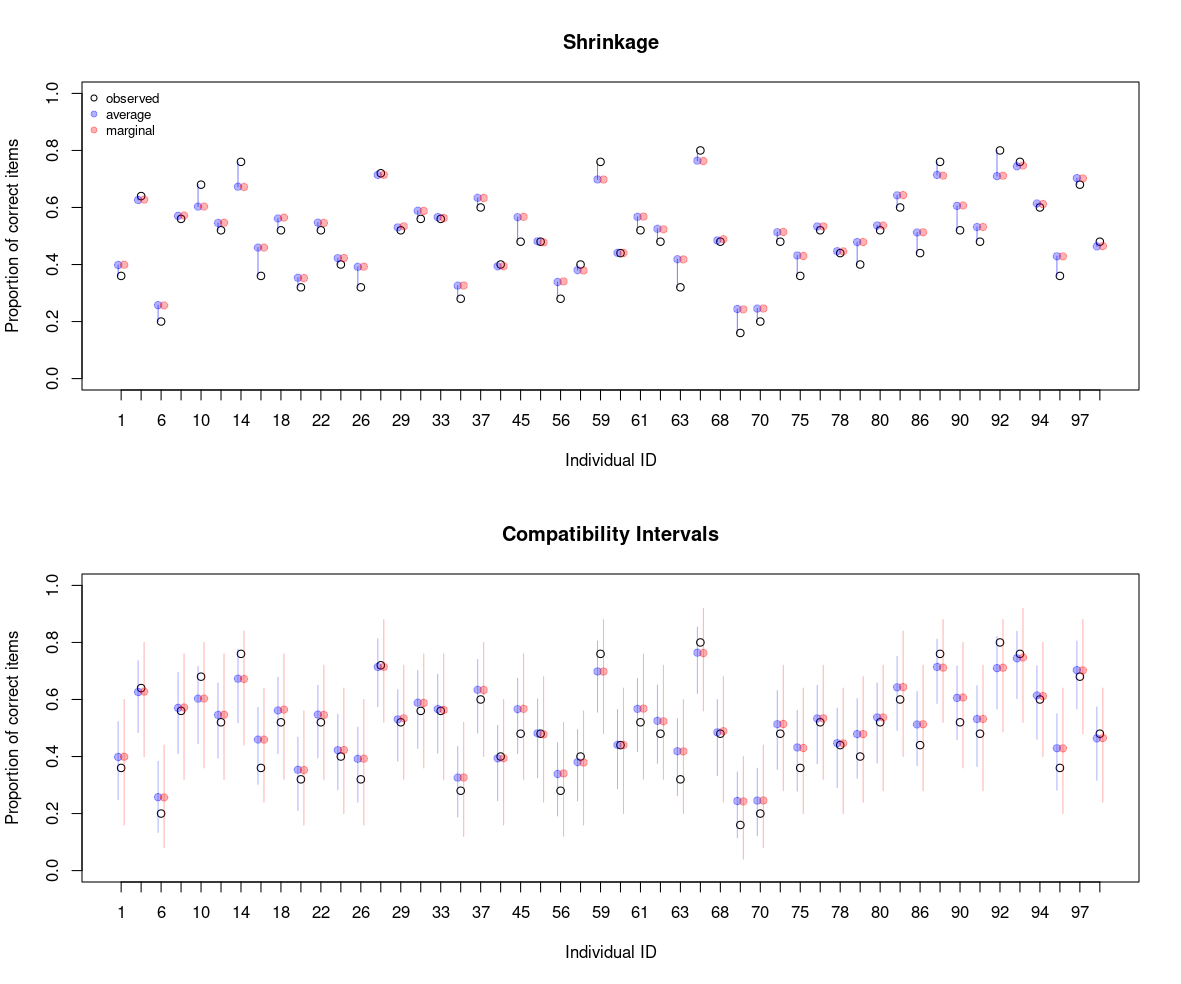
\includegraphics[width=0.9\linewidth]{FOLV_NC_J100_Ndata4_HitRate_ind}
	%
	\caption[First-order latent variable model (FOLV). Sample size $100$, replica number $4$. Non-centered parametrization. Individual predictive plot.]%
	{First-order latent variable model (FOLV). Sample size $100$, replica number $4$. Non-centered parametrization. Individual predictive plot.}
	\label{fig:FOLV_NC_hitrate_ind}
\end{figure}

On the other hand, for the same model, figures \ref{fig:FOLV_CE_ICC} and \ref{fig:FOLV_CE_IIF} (appendix) show the true, average, and marginal items characteristic curves, and item information functions. From the figures, we notice the model manages to reproduce rather well the true ICC and IIF curves. This means that the model allow us to correctly recover the item's psychometric characteristics, a trait of high relevance for the development of instruments.
%
\begin{figure}[H]
	\centering
	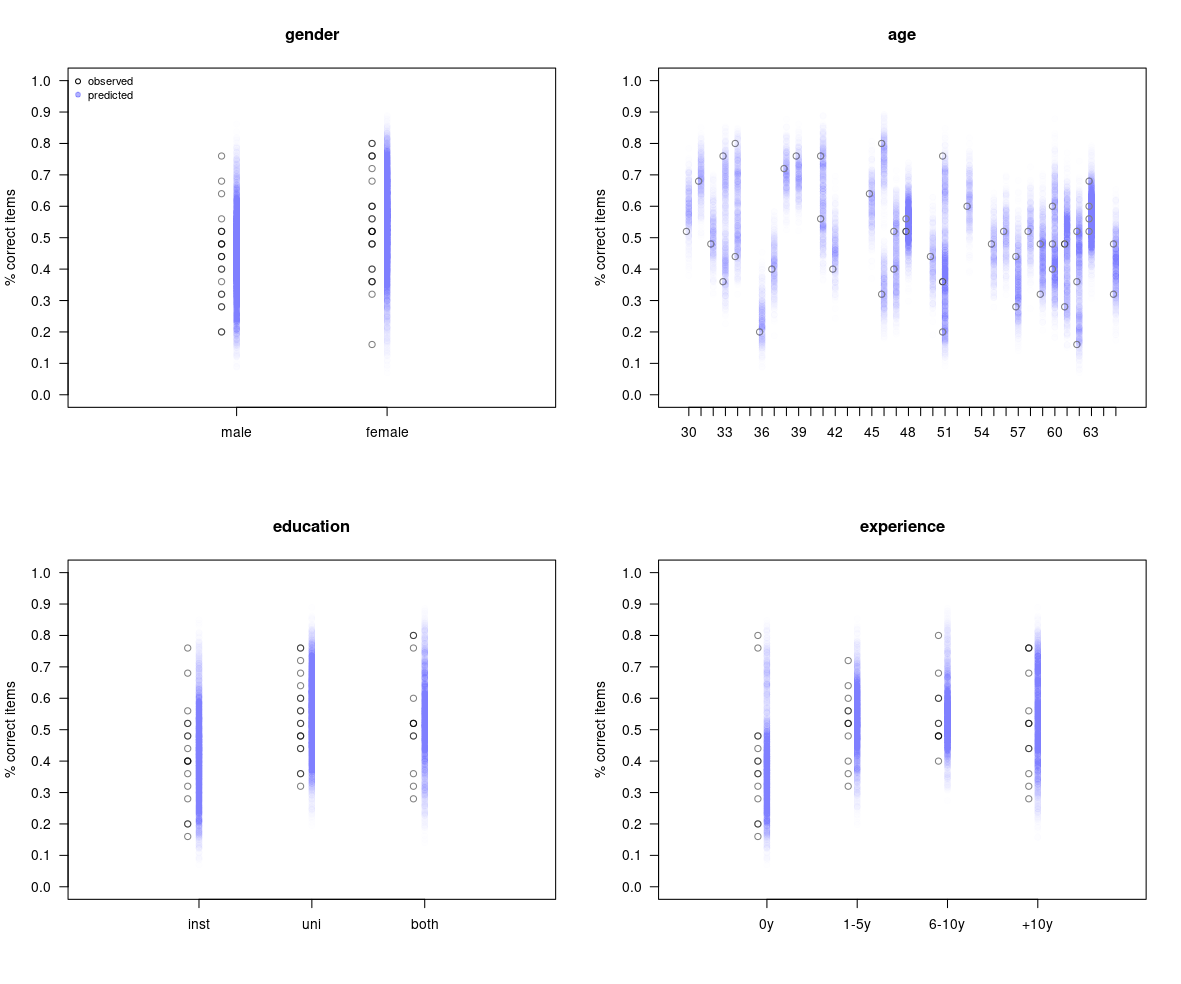
\includegraphics[width=1\linewidth]{FOLV_NC_J100_Ndata4_HitRate_var}
	%
	\caption[First-order latent variable model (FOLV). Sample size $100$, replica number $4$. Non-centered parametrization. Individual predictive plot per covariate.]%
	{First-order latent variable model (FOLV). Sample size $100$, replica number $4$. Non-centered parametrization. Individual predictive plot per covariate.}
	\label{fig:FOLV_NC_hitrate_var}
\end{figure}

Figures \ref{fig:SOLV_NC_hitrate_ind} through \ref{fig:SOLV_CE_IIF} (appendix) show the SOLV model obtained similar results. Moreover, a careful inspection of similar plots for all replicas, sample sizes, and parametrizations\footnote{To inspect the prediction plot follow the github accompanying page detailed in Appendix \ref{sub_sect:retro_accuracy}.} revealed the preceding patterns of retrodictive accuracy are consistent across the conditions, with no apparent difference between the CP and NCP. This results also resonates with the patterns obtained in the previous section.

Finally, tables \ref{tab:FOLV_accuracy} and \ref{tab:SOLV_accuracy} further confirm that no difference in the individuals' retrodictive accuracy is observed between the CP and NCP, under the FOLV or SOLV model. Moreover, they reveal the predictive uncertainty is higher within rather than between the replicas, that is, the models predicted the data in a similar manner across replicas. A similar behavior is observed for the items' retrodictive accuracy, as tables \ref{tab:FOLV_accuracy_items} and \ref{tab:SOLV_accuracy_items} show.
%
\begin{table}[H]
	\centering
	\begin{tabular}{rlrrrrrrrrr}
		\hline
		& & Sample && \multicolumn{3}{c}{ $\overline{\text{RMSE}}_{W}$ } && \multicolumn{3}{c}{ $\text{RMSE}_{B}$ } \\
		\cmidrule(rl){5-7} \cmidrule(rl){9-11}  
		& Parametrization & size  && mean & min & max && mean & min & max \\ 
		\hline\hline
		1 & CP & 100 && 0.113 & 0.106 & 0.120 && 0.041 & 0.018 & 0.058 \\ 
		2 & CP & 250 && 0.114 & 0.107 & 0.127 && 0.041 & 0.023 & 0.070 \\
		3 & CP & 500 && 0.112 & 0.104 & 0.125 && 0.041 & 0.015 & 0.076 \\
		%
		\hline
		%
		4 & NCP & 100 && 0.113 & 0.106 & 0.121 && 0.041 & 0.018 & 0.059 \\ 
		5 & NCP & 250 && 0.114 & 0.107 & 0.125 && 0.041 & 0.023 & 0.068 \\ 
		6 & NCP & 500 && 0.112 & 0.105 & 0.126 && 0.041 & 0.015 & 0.077 \\
		\hline
	\end{tabular}
	\caption[First-order latent variable model (FOLV). Centered and non-centered parametrization. Within and between replicas individual predictive RMSE.]%
	{First-order latent variable model (FOLV). Centered and non-centered parametrization. Within and between replicas individual predictive RMSE.}
	\label{tab:FOLV_accuracy}
\end{table}
%
\begin{table}[H]
	\centering
	\begin{tabular}{rlrrrrrrrrr}
		\hline
		&  & Sample && \multicolumn{3}{c}{ $\overline{\text{RMSE}}_{W}$ } && \multicolumn{3}{c}{ $\text{RMSE}_{B}$ } \\
		\cmidrule(rl){5-7} \cmidrule(rl){9-11}  
		& Parametrization & size  && mean & min & max && mean & min & max \\ 
		\hline\hline
		1 & CP & 100 && 0.112 & 0.106 & 0.117 && 0.034 & 0.015 & 0.050 \\ 
		2 & CP & 250 && 0.112 & 0.107 & 0.122 && 0.035 & 0.018 & 0.059 \\ 
		3 & CP & 500 && 0.111 & 0.104 & 0.122 && 0.036 & 0.015 & 0.068 \\ 
		%
		\hline
		%
		4 & NCP & 100 && 0.112 & 0.106 & 0.117 && 0.034 & 0.015 & 0.050 \\
		5 & NCP & 250 && 0.112 & 0.106 & 0.121 && 0.035 & 0.018 & 0.057 \\
		6 & NCP & 500 && 0.111 & 0.105 & 0.122 && 0.036 & 0.014 & 0.068 \\ 
		\hline
	\end{tabular}
	\caption[Second-order latent variable model (SOLV). Centered and non-centered parametrization. Within and between replicas individual predictive RMSE.]%
	{Second-order latent variable model (SOLV). Centered and non-centered parametrization. Within and between replicas individual predictive RMSE.}
	\label{tab:SOLV_accuracy}
\end{table}

%%%%%%%%%%%%%%%%%%%%%%%%%%%%%%%%%%%%%%%%%%%%%%%%%%%%%%%%%%%%%%%%%%%%%%%

\subsection{Time}

Although the assessment and comparison of the MCMC procedure's running time is not one of the main goals of the study, the researcher believes it is useful to report them, as they could serve as a benchmark of comparison for future developments.

Tables \ref{tab:FOLV_time} and \ref{tab:SOLV_time} report the CP and NCP MCMC running time, for the FOLV and SOLV model, respectively. As the reader can recall, we decided to use $10$ replicas for each combination of model, parametrization and sample size. On each replica, the posterior distribution of the parameters was approximated through an HMC procedure with $3$ chains (run in parallel), with $2,000$ iterations per chain. From the tables, we can see the NCP was faster than the CP for the smallest sample sizes ($100$ and $250$).  However, the differences in running time got smaller as the sample size increased. This was true for both type of models. 

The NCP being slightly faster than the CP is important, as the non-centered parametrization is more complex, and requires the sampling of more parameters than the centered counterpart. This just means that improving the performance of the MCMC, through a more complex model as the NCP, does not come with a cost on running time.
%
\begin{table}[H]
	\centering
	\begin{tabular}{rlrrrr}
		\hline
		\multicolumn{3}{c}{ }& \multicolumn{3}{c}{ Time (min.) } \\ 
		\cmidrule(rl){4-6} 
		& Parametrization & Sample & mean & min & max \\ 
		\hline\hline
		1 & CP & 100 & 4.80 & 1.89 & 7.56 \\ 
		2 & CP & 250 & 7.85 & 5.60 & 16.57 \\ 
		3 & CP & 500 & 19.15 & 17.20 & 22.53 \\ 
		%
		\hline
		%
		4 & NCP & 100 & 1.94 & 1.74 & 2.23 \\ 
		5 & NCP & 250 & 7.18 & 6.78 & 8.40 \\ 
		6 & NCP & 500 & 22.38 & 20.12 & 28.62 \\
		\hline
	\end{tabular}
	\caption[First-order latent variable model (FOLV). Running time statistics.]%
	{First-order latent variable model (FOLV). Running time statistics.} 
	\label{tab:FOLV_time}
\end{table}
%
\begin{table}[H]
	\centering
	\begin{tabular}{rlrrrr}
		\hline
		\multicolumn{3}{c}{ }& \multicolumn{3}{c}{ Time (min.) } \\ 
		\cmidrule(rl){4-6} 
		& Parametrization & Sample & mean & min & max \\ 
		\hline\hline
		1 & CP & 100 & 4.04 & 1.39 & 8.55 \\ 
		2 & CP & 250 & 7.13 & 5.22 & 11.49 \\ 
		3 & CP & 500 & 16.14 & 14.45 & 19.73 \\ 
		%
		\hline
		%
		4 & NCP & 100 & 1.87 & 1.62 & 2.28 \\ 
		5 & NCP & 250 & 5.92 & 5.20 & 6.79 \\ 
		6 & NCP & 500 & 16.58 & 13.37 & 18.26 \\
		\hline
	\end{tabular}
	\caption[Second-order latent variable model (SOLV). Running time statistics.]%
	{Second-order latent variable model (SOLV). Running time statistics.} 
	\label{tab:SOLV_time}
\end{table}
